%**************************************%
%* Generated from MathBook XML source *%
%*    on 2016-08-14T13:22:57-04:00    *%
%*                                    *%
%*   http://mathbook.pugetsound.edu   *%
%*                                    *%
%**************************************%
\documentclass[10pt,]{book}
%% Load geometry package to allow page margin adjustments
\usepackage{geometry}
\geometry{letterpaper,total={5.0in,9.0in}}
%% Custom Preamble Entries, early (use latex.preamble.early)
%% Inline math delimiters, \(, \), need to be robust
%% 2016-01-31:  latexrelease.sty  supersedes  fixltx2e.sty
%% If  latexrelease.sty  exists, bugfix is in kernel
%% If not, bugfix is in  fixltx2e.sty
%% See:  https://tug.org/TUGboat/tb36-3/tb114ltnews22.pdf
%% and read "Fewer fragile commands" in distribution's  latexchanges.pdf
\IfFileExists{latexrelease.sty}{}{\usepackage{fixltx2e}}
%% Page Layout Adjustments (latex.geometry)
%% This LaTeX file may be compiled with pdflatex, xelatex, or lualatex
%% The following provides engine-specific capabilities
%% Generally, xelatex and lualatex will do better languages other than US English
%% You can pick from the conditional if you will only ever use one engine
\usepackage{ifthen}
\usepackage{ifxetex,ifluatex}
\ifthenelse{\boolean{xetex} \or \boolean{luatex}}{%
%% begin: xelatex and lualatex-specific configuration
%% fontspec package will make Latin Modern (lmodern) the default font
\ifxetex\usepackage{xltxtra}\fi
\usepackage{fontspec}
%% realscripts is the only part of xltxtra relevant to lualatex 
\ifluatex\usepackage{realscripts}\fi
%% 
%% Extensive support for other languages
\usepackage{polyglossia}
\setdefaultlanguage{english}
%% Magyar (Hungarian)
\setotherlanguage{magyar}
%% Spanish
\setotherlanguage{spanish}
%% Vietnamese
\setotherlanguage{vietnamese}
%% end: xelatex and lualatex-specific configuration
}{%
%% begin: pdflatex-specific configuration
%% translate common Unicode to their LaTeX equivalents
%% Also, fontenc with T1 makes CM-Super the default font
%% (\input{ix-utf8enc.dfu} from the "inputenx" package is possible addition (broken?)
\usepackage[T1]{fontenc}
\usepackage[utf8]{inputenc}
%% end: pdflatex-specific configuration
}
%% Monospace font: Inconsolata (zi4)
%% Sponsored by TUG: http://levien.com/type/myfonts/inconsolata.html
%% See package documentation for excellent instructions
%% One caveat, seem to need full file name to locate OTF files
%% Loads the "upquote" package as needed, so we don't have to
%% Upright quotes might come from the  textcomp  package, which we also use
%% We employ the shapely \ell to match Google Font version
%% pdflatex: "varqu" option produces best upright quotes
%% xelatex,lualatex: add StylisticSet 1 for shapely \ell
%% xelatex,lualatex: add StylisticSet 2 for plain zero
%% xelatex,lualatex: we add StylisticSet 3 for upright quotes
%% 
\ifthenelse{\boolean{xetex} \or \boolean{luatex}}{%
%% begin: xelatex and lualatex-specific monospace font
\usepackage{zi4}
\setmonofont[BoldFont=Inconsolatazi4-Bold.otf,StylisticSet={1,3}]{Inconsolatazi4-Regular.otf}
%% end: xelatex and lualatex-specific monospace font
}{%
%% begin: pdflatex-specific monospace font
\usepackage[varqu]{zi4}
%% end: pdflatex-specific monospace font
}
%% Symbols, align environment, bracket-matrix
\usepackage{amsmath}
\usepackage{amssymb}
%% allow more columns to a matrix
%% can make this even bigger by overriding with  latex.preamble.late  processing option
\setcounter{MaxMatrixCols}{30}
%%
%% Color support, xcolor package
%% Always loaded.  Used for:
%% mdframed boxes, add/delete text, author tools
\PassOptionsToPackage{usenames,dvipsnames,svgnames,table}{xcolor}
\usepackage{xcolor}
%%
%% Semantic Macros
%% To preserve meaning in a LaTeX file
%% Only defined here if required in this document
%% Used for inline definitions of terms
\newcommand{\terminology}[1]{\textbf{#1}}
%% Subdivision Numbering, Chapters, Sections, Subsections, etc
%% Subdivision numbers may be turned off at some level ("depth")
%% A section *always* has depth 1, contrary to us counting from the document root
%% The latex default is 3.  If a larger number is present here, then
%% removing this command may make some cross-references ambiguous
%% The precursor variable $numbering-maxlevel is checked for consistency in the common XSL file
\setcounter{secnumdepth}{3}
%% Environments with amsthm package
%% Theorem-like environments in "plain" style, with or without proof
\usepackage{amsthm}
\theoremstyle{plain}
%% Numbering for Theorems, Conjectures, Examples, Figures, etc
%% Controlled by  numbering.theorems.level  processing parameter
%% Always need a theorem environment to set base numbering scheme
%% even if document has no theorems (but has other environments)
\newtheorem{theorem}{Theorem}[section]
%% Only variants actually used in document appear here
%% Style is like a theorem, and for statements without proofs
%% Numbering: all theorem-like numbered consecutively
%% i.e. Corollary 4.3 follows Theorem 4.2
\newtheorem{algorithm}[theorem]{Algorithm}
%% Definition-like environments, normal text
%% Numbering is in sync with theorems, etc
\theoremstyle{definition}
\newtheorem{definition}[theorem]{Definition}
%% Remark-like environments, normal text
%% Numbering is in sync with theorems, etc
\theoremstyle{definition}
\newtheorem{note}[theorem]{Note}
%% Example-like environments, normal text
%% Numbering is in sync with theorems, etc
\theoremstyle{definition}
\newtheorem{example}[theorem]{Example}
%% Miscellaneous environments, normal text
%% Numbering for inline exercises and lists is in sync with theorems, etc
\theoremstyle{definition}
\newtheorem{exercise}[theorem]{Exercise}
%% Localize LaTeX supplied names (possibly none)
\renewcommand*{\chaptername}{Chapter}
%% For improved tables
\usepackage{array}
%% Some extra height on each row is desirable, especially with horizontal rules
%% Increment determined experimentally
\setlength{\extrarowheight}{0.2ex}
%% Define variable thickness horizontal rules, full and partial
%% Thicknesses are 0.03, 0.05, 0.08 in the  booktabs  package
\makeatletter
\newcommand{\hrulethin}  {\noalign{\hrule height 0.04em}}
\newcommand{\hrulemedium}{\noalign{\hrule height 0.07em}}
\newcommand{\hrulethick} {\noalign{\hrule height 0.11em}}
%% We preserve a copy of the \setlength package before other
%% packages (extpfeil) get a chance to load packages that redefine it
\let\oldsetlength\setlength
\newlength{\Oldarrayrulewidth}
\newcommand{\crulethin}[1]%
{\noalign{\global\oldsetlength{\Oldarrayrulewidth}{\arrayrulewidth}}%
\noalign{\global\oldsetlength{\arrayrulewidth}{0.04em}}\cline{#1}%
\noalign{\global\oldsetlength{\arrayrulewidth}{\Oldarrayrulewidth}}}%
\newcommand{\crulemedium}[1]%
{\noalign{\global\oldsetlength{\Oldarrayrulewidth}{\arrayrulewidth}}%
\noalign{\global\oldsetlength{\arrayrulewidth}{0.07em}}\cline{#1}%
\noalign{\global\oldsetlength{\arrayrulewidth}{\Oldarrayrulewidth}}}
\newcommand{\crulethick}[1]%
{\noalign{\global\oldsetlength{\Oldarrayrulewidth}{\arrayrulewidth}}%
\noalign{\global\oldsetlength{\arrayrulewidth}{0.11em}}\cline{#1}%
\noalign{\global\oldsetlength{\arrayrulewidth}{\Oldarrayrulewidth}}}
%% Single letter column specifiers defined via array package
\newcolumntype{A}{!{\vrule width 0.04em}}
\newcolumntype{B}{!{\vrule width 0.07em}}
\newcolumntype{C}{!{\vrule width 0.11em}}
\makeatother
%% Figures, Tables, Listings, Floats
%% The [H]ere option of the float package fixes floats in-place,
%% in deference to web usage, where floats are totally irrelevant
%% We re/define the figure, table and listing environments, if used
%%   1) New mbxfigure and/or mbxtable environments are defined with float package
%%   2) Standard LaTeX environments redefined to use new environments
%%   3) Standard LaTeX environments redefined to step theorem counter
%%   4) Counter for new environments is set to the theorem counter before caption
%% You can remove all this figure/table setup, to restore standard LaTeX behavior
%% HOWEVER, numbering of figures/tables AND theorems/examples/remarks, etc
%% WILL ALL de-synchronize with the numbering in the HTML version
%% You can remove the [H] argument of the \newfloat command, to allow flotation and 
%% preserve numbering, BUT the numbering may then appear "out-of-order"
\usepackage{float}
\usepackage[bf]{caption} % http://tex.stackexchange.com/questions/95631/defining-a-new-type-of-floating-environment 
\usepackage{newfloat}
% Figure environment setup so that it no longer floats
\SetupFloatingEnvironment{figure}{fileext=lof,placement={H},within=section,name=Figure}
% figures have the same number as theorems: http://tex.stackexchange.com/questions/16195/how-to-make-equations-figures-and-theorems-use-the-same-numbering-scheme 
\makeatletter
\let\c@figure\c@theorem
\makeatother
% Table environment setup so that it no longer floats
\SetupFloatingEnvironment{table}{fileext=lot,placement={H},within=section,name=Table}
% tables have the same number as theorems: http://tex.stackexchange.com/questions/16195/how-to-make-equations-figures-and-theorems-use-the-same-numbering-scheme 
\makeatletter
\let\c@table\c@theorem
\makeatother
%% Raster graphics inclusion, wrapped figures in paragraphs
%% \resizebox sometimes used for images in side-by-side layout
\usepackage{graphicx}
%%
%% Program listing support, for inline code, Sage code
\usepackage{listings}
%% We define the listings font style to be the default "ttfamily"
%% To fix hyphens/dashes rendered in PDF as fancy minus signs by listing
%% http://tex.stackexchange.com/questions/33185/listings-package-changes-hyphens-to-minus-signs
\makeatletter
\lst@CCPutMacro\lst@ProcessOther {"2D}{\lst@ttfamily{-{}}{-{}}}
\@empty\z@\@empty
\makeatother
\ifthenelse{\boolean{xetex}}{}{%
%% begin: pdflatex-specific listings configuration
%% translate U+0080 - U+00F0 to their textmode LaTeX equivalents
%% Data originally from https://www.w3.org/Math/characters/unicode.xml, 2016-07-23
%% Lines marked in XSL with "$" were converted from mathmode to textmode
\lstset{extendedchars=true}
\lstset{literate={ }{{~}}{1}{¡}{{\textexclamdown }}{1}{¢}{{\textcent }}{1}{£}{{\textsterling }}{1}{¤}{{\textcurrency }}{1}{¥}{{\textyen }}{1}{¦}{{\textbrokenbar }}{1}{§}{{\textsection }}{1}{¨}{{\textasciidieresis }}{1}{©}{{\textcopyright }}{1}{ª}{{\textordfeminine }}{1}{«}{{\guillemotleft }}{1}{¬}{{\textlnot }}{1}{­}{{\-}}{1}{®}{{\textregistered }}{1}{¯}{{\textasciimacron }}{1}{°}{{\textdegree }}{1}{±}{{\textpm }}{1}{²}{{\texttwosuperior }}{1}{³}{{\textthreesuperior }}{1}{´}{{\textasciiacute }}{1}{µ}{{\textmu }}{1}{¶}{{\textparagraph }}{1}{·}{{\textperiodcentered }}{1}{¸}{{\c{}}}{1}{¹}{{\textonesuperior }}{1}{º}{{\textordmasculine }}{1}{»}{{\guillemotright }}{1}{¼}{{\textonequarter }}{1}{½}{{\textonehalf }}{1}{¾}{{\textthreequarters }}{1}{¿}{{\textquestiondown }}{1}{À}{{\`{A}}}{1}{Á}{{\'{A}}}{1}{Â}{{\^{A}}}{1}{Ã}{{\~{A}}}{1}{Ä}{{\"{A}}}{1}{Å}{{\AA }}{1}{Æ}{{\AE }}{1}{Ç}{{\c{C}}}{1}{È}{{\`{E}}}{1}{É}{{\'{E}}}{1}{Ê}{{\^{E}}}{1}{Ë}{{\"{E}}}{1}{Ì}{{\`{I}}}{1}{Í}{{\'{I}}}{1}{Î}{{\^{I}}}{1}{Ï}{{\"{I}}}{1}{Ð}{{\DH }}{1}{Ñ}{{\~{N}}}{1}{Ò}{{\`{O}}}{1}{Ó}{{\'{O}}}{1}{Ô}{{\^{O}}}{1}{Õ}{{\~{O}}}{1}{Ö}{{\"{O}}}{1}{×}{{\texttimes }}{1}{Ø}{{\O }}{1}{Ù}{{\`{U}}}{1}{Ú}{{\'{U}}}{1}{Û}{{\^{U}}}{1}{Ü}{{\"{U}}}{1}{Ý}{{\'{Y}}}{1}{Þ}{{\TH }}{1}{ß}{{\ss }}{1}{à}{{\`{a}}}{1}{á}{{\'{a}}}{1}{â}{{\^{a}}}{1}{ã}{{\~{a}}}{1}{ä}{{\"{a}}}{1}{å}{{\aa }}{1}{æ}{{\ae }}{1}{ç}{{\c{c}}}{1}{è}{{\`{e}}}{1}{é}{{\'{e}}}{1}{ê}{{\^{e}}}{1}{ë}{{\"{e}}}{1}{ì}{{\`{\i}}}{1}{í}{{\'{\i}}}{1}{î}{{\^{\i}}}{1}{ï}{{\"{\i}}}{1}{ð}{{\dh }}{1}{ñ}{{\~{n}}}{1}{ò}{{\`{o}}}{1}{ó}{{\'{o}}}{1}{ô}{{\^{o}}}{1}{õ}{{\~{o}}}{1}{ö}{{\"{o}}}{1}{÷}{{\textdiv }}{1}{ø}{{\o }}{1}{ù}{{\`{u}}}{1}{ú}{{\'{u}}}{1}{û}{{\^{u}}}{1}{ü}{{\"{u}}}{1}{ý}{{\'{y}}}{1}{þ}{{\th }}{1}{ÿ}{{\"{y}}}{1}}
%% end: pdflatex-specific listings configuration
}
%% End of generic listing adjustments
%% Generic input, listings package: boxed, white, line breaking, language per instance
%% Colors match a subset of Google prettify "Default" style
%% Set latex.print='yes" to get all black
%% http://code.google.com/p/google-code-prettify/source/browse/trunk/src/prettify.css
\definecolor{identifiers}{rgb}{0.375,0,0.375}
\definecolor{comments}{rgb}{0.5,0,0}
\definecolor{strings}{rgb}{0,0.5,0}
\definecolor{keywords}{rgb}{0,0,0.5}
\lstdefinestyle{genericinput}{breaklines=true,breakatwhitespace=true,columns=fixed,frame=single,xleftmargin=4ex,xrightmargin=4ex,
basicstyle=\small\ttfamily,identifierstyle=\color{identifiers},commentstyle=\color{comments},stringstyle=\color{strings},keywordstyle=\color{keywords}}
%% More flexible list management, esp. for references and exercises
%% But also for specifying labels (i.e. custom order) on nested lists
\usepackage{enumitem}
%% Lists of references in their own section, maximum depth 1
\newlist{referencelist}{description}{4}
\setlist[referencelist]{leftmargin=!,labelwidth=!,labelsep=0ex,itemsep=1.0ex,topsep=1.0ex,partopsep=0pt,parsep=0pt}
%% Lists of exercises in their own section, maximum depth 4
\newlist{exerciselist}{description}{4}
\setlist[exerciselist]{leftmargin=0pt,itemsep=1.0ex,topsep=1.0ex,partopsep=0pt,parsep=0pt}
%% Indented groups of exercises within an exercise section, maximum depth 4
\newlist{exercisegroup}{description}{4}
\setlist[exercisegroup]{leftmargin=2em,labelindent=2em,itemsep=1.0ex,topsep=1.0ex,partopsep=0pt,parsep=0pt}
%% Support for index creation
%% imakeidx package does not require extra pass (as with makeidx)
%% We set the title of the "Index" section via a keyword
%% And we provide language support for the "see" phrase
\usepackage{imakeidx}
\makeindex[title=Index, intoc=true]
\renewcommand{\seename}{see}
%% Package for tables spanning several pages
\usepackage{longtable}
%% hyperref driver does not need to be specified
\usepackage{hyperref}
%% configure hyperref's  \url  to match listings' inline verbatim
\renewcommand\UrlFont{\small\ttfamily}
%% Hyperlinking active in PDFs, all links solid and blue
\hypersetup{colorlinks=true,linkcolor=blue,citecolor=blue,filecolor=blue,urlcolor=blue}
\hypersetup{pdftitle={Applied Discrete Structures}}
%% If you manually remove hyperref, leave in this next command
\providecommand\phantomsection{}
%% If tikz has been loaded, replace ampersand with \amp macro
%% extpfeil package for certain extensible arrows,
%% as also provided by MathJax extension of the same name
%% NB: this package loads mtools, which loads calc, which redefines
%%     \setlength, so it can be removed if it seems to be in the 
%%     way and your math does not use:
%%     
%%     \xtwoheadrightarrow, \xtwoheadleftarrow, \xmapsto, \xlongequal, \xtofrom
%%     
%%     we have had to be extra careful with variable thickness
%%     lines in tables, and so also load this package late
\usepackage{extpfeil}
%% Custom Preamble Entries, late (use latex.preamble.late)
%% Begin: Author-provided macros
%% (From  docinfo/macros  element)
%% Plus three from MBX for XML characters
\newcommand{\identity}{\mathrm{id}}
\newcommand{\notdivide}{{\not{\mid}}}
\newcommand{\notsubset}{\not\subset}
\newcommand{\lcm}{\operatorname{lcm}}
\newcommand{\gf}{\operatorname{GF}}
\newcommand{\inn}{\operatorname{Inn}}
\newcommand{\aut}{\operatorname{Aut}}
\newcommand{\Hom}{\operatorname{Hom}}
\newcommand{\cis}{\operatorname{cis}}
\newcommand{\chr}{\operatorname{char}}
\newcommand{\Null}{\operatorname{Null}}
\newcommand{\lt}{ < }
\newcommand{\gt}{ > }
\newcommand{\amp}{ & }
%% End: Author-provided macros
%% Title page information for book
\title{Applied Discrete Structures}
\author{Al Doerr\\
Department of Mathematical Sciences\\
University of Massachusetts Lowell\\
\href{mailto:}{\nolinkurl{}}
\and
Ken Levasseur\\
Department of Mathematical Sciences\\
University of Massachusetts Lowell\\
\href{mailto:kenneth_levasseur@uml.edu}{\nolinkurl{kenneth_levasseur@uml.edu}}
}
\date{September, 2016}
\begin{document}
\frontmatter
%% begin: half-title
\thispagestyle{empty}
{\centering
\vspace*{0.28\textheight}
{\Huge Applied Discrete Structures}\\}
\clearpage
%% end:   half-title
%% begin: adcard
\thispagestyle{empty}
\null%
\clearpage
%% end:   adcard
%% begin: title page
%% Inspired by Peter Wilson's "titleDB" in "titlepages" CTAN package
\thispagestyle{empty}
{\centering
\vspace*{0.14\textheight}
{\Huge Applied Discrete Structures}\\[3\baselineskip]
{\Large Al Doerr}\\[0.5\baselineskip]
{\Large University of Massachusetts Lowell}\\[3\baselineskip]
{\Large Ken Levasseur}\\[0.5\baselineskip]
{\Large University of Massachusetts Lowell}\\[3\baselineskip]
{\Large September, 2016}\\}
\clearpage
%% end:   title page
%% begin: copyright-page
\thispagestyle{empty}
\vspace*{\stretch{2}}
\noindent\textcopyright\ 2016\quad{}Al Doerr, Ken Levasseur\\[0.5\baselineskip]
Applied Discrete Structures by Alan Doerr and Kenneth Levasseur is licensed under a Creative Commons Attribution-NonCommercial-ShareAlike 3.0 United States License. You are free to Share: copy and redistribute the material in any medium or format; Adapt: remix, transform, and build upon the material. You may not use the material for commercial purposes.  The licensor cannot revoke these freedoms as long as you follow the license terms.
			\par
\vspace*{\stretch{1}}
\null\clearpage
%% end:   copyright-page
%% begin: acknowledgement
\chapter*{Acknowledgements}\label{acknowledgement-1}
\addcontentsline{toc}{chapter}{Acknowledgements}
I would like to thank Rob Beezer, David Farmer and other participants on the \href{https://groups.google.com/forum/?fromgroups#!forum/mathbook-xml-support}{mathbook-xml-support group} for their guidance and work on MathBook XML.  Thanks to the Pedagogy Subcommittee of the UMass Lowell Transformational Education Committee for their financial assistance in helping getting this project started.%
%% end:   acknowledgement
%% begin: preface
\chapter*{Preface}\label{preface-1}
\addcontentsline{toc}{chapter}{Preface}
This version of \emph{Applied Discrete Structures} is being developed using \emph{Mathbook XML}, A lightweight XML application for authors of scientific articles, textbooks and monographs initiated by Rob Beezer, U. of Puget Sound.  %
\par
Sage (\href{http://sagemath.org}{sagemath.org}) is a free, open source, software system for advanced mathematics.  Sage can be used either on your own computer, a local server, or on SageMathCloud (\href{https://cloud.sagemath.com}{https://cloud.sagemath.com}). %
\par\hfill\begin{tabular}{l@{}}
Ken Levasseur\\
Lowell MA
\end{tabular}\\\par
%% end:   preface
%% begin: table of contents
\setcounter{tocdepth}{1}
\renewcommand*\contentsname{Contents}
\tableofcontents
%% end:   table of contents
\mainmatter
\typeout{************************************************}
\typeout{Chapter 1 Relations}
\typeout{************************************************}
\chapter[Relations]{Relations}\label{chapter_6}
\typeout{************************************************}
\typeout{Introduction  }
\typeout{************************************************}
One understands a set of objects completely only if the structure of that set is made clear by the interrelationships between its elements. For example, the individuals in a crowd can be compared by height, by age, or through any number of other criteria. In mathematics, such comparisons are called relations. The goal of this chapter is to develop the language, tools, and concepts of relations.%
\typeout{************************************************}
\typeout{Section 1.1 Basic Definitions}
\typeout{************************************************}
\section[Basic Definitions]{Basic Definitions}\label{s-basic-definitions}
In Chapter 1 we introduced the concept of the Cartesian product of sets. Let's assume that a person owns three shirts and two pairs of slacks. More
precisely, let \(A = \{\textrm{blue shirt}, \textrm{tan shirt}, \textrm{mint green shirt}\}\) and \(B = \{\textrm{grey slacks}, \textrm{tan slacks}\}\). Then \(A\times B\) is the set of all six possible combinations of shirts and slacks that the individual could wear. However, an individual may wish to restrict himself or herself to combinations which are color coordinated, or ``related.'' This may not be all possible pairs in \(A\times B\) but will certainly be a subset of \(A\times B\). For example, one such subset may be \(\{(\textrm{blue shirt}, \textrm{grey slacks}), (\textrm{blue shirt},  \textrm{tan slacks}), (\textrm{mint green shirt}, \textrm{tan slacks})\}\).%
\begin{definition}[Relation]\label{Relation}
\index{Relation} Let A and B be sets. A relation from A into B is any subset of \(A\times B\).%
\end{definition}
\begin{example}[A simple example]\label{ex-simple-relation}
Let \(A = \{1, 2, 3\}\) and \(B = \{4, 5\}\). Then \(\{(1, 4), (2, 4), (3, 5)\}\) is a relation from \(A\) into \(B\). Of course, there are many others we could describe; 64, to be exact.%
\end{example}
\begin{example}[Divisibility Example]\label{ex-divides-example}
 Let \(A = \{2, 3, 5, 6\}\) and define a relation \(r\) from \(A\) into \(A\) by \((a, b) \in r\) if and only if \(a\) divides evenly into \(b\). The set of pairs that qualify for membership is \(r = \{(2, 2), (3, 3), (5, 5), (6, 6), (2, 6), (3, 6)\}\).
%
\end{example}
\begin{definition}[Relation on a Set]\label{relation-on-a-set}
\index{Relation on a Set}A relation from a set A into itself is called a relation on A.%
\end{definition}
\par
The relation ``divides'' in \hyperref[ex-divides-example]{Example~\ref{ex-divides-example}} is will appear throughout the book. Here is a general definition on the whole set of integers.%
\begin{definition}[Divides]\label{Divides}
\index{Divides}\label{notation-1}
Let \(a, b \in \mathbb{Z}\).  
We say that \(a\) divides \(b\), denoted \(a \mid b\),  if and only if there exists an integer \(k\) such that \(a k = b\).%
\end{definition}
\par
Be very careful in writing about the relation ``divides.''  The vertical line symbol use for this relation, if written carelessly, can look like division.  While \(a \mid b\) is either true or false, \(a/b\) is a number. %
\par
Based on the equation \(a k = b\), we can say that \(a|b\) is equivalent to \(k= \frac{b}{a}\), or \(a\) divides evenly into \(b\). In fact the ``divides'' is short for ``divides evenly into.'' You might find the equation \(k= \frac{b}{a}\) initially easier to understand, but in the long run we will find the equation \(a k = b\) more convenient. %
\par
Sometimes it is helpful to illustrate a relation with a graph. Consider \hyperref[ex-simple-relation]{Example~\ref{ex-simple-relation}}.  A graph of \(r\) can be drawn as in \hyperref[graph-6-1-1-relation]{Figure~\ref{graph-6-1-1-relation}}. The arrows indicate that 1 is related to 4 under \(r\). Also, 2 is related to 4 under \(r\), and 3 is related to 5, while the upper arrow denotes that \(r\) is a relation from the whole set \(A\) into the set \(B\). %
\leavevmode%
\begin{figure}
\centering
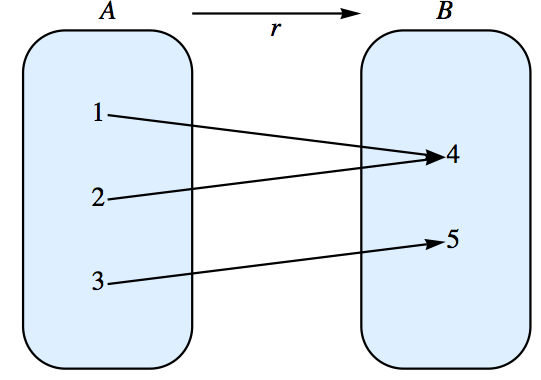
\includegraphics[width=1\linewidth]{images/graph-6-1-relation-graph.png}
\caption{The graph of a relation\label{graph-6-1-1-relation}}
\end{figure}
\par
A typical element in a relation \(r\) is an ordered pair \((x, y)\). In some cases, \(r\) can be described by actually listing the pairs which are in \(r\), as in the previous examples. This may not be convenient if \(r\) is relatively large. Other notations are used with certain well-known relations. Consider the ``less than or equal'' relation on the real numbers. We could define it as a set of ordered pairs this way:
\[\le = \{(x, y) | x \leq  y\}\].
However, the notation \(x \leq  y\) is clear and self-explanatory; it is a more natural, and hence preferred, notation to use than \((x, y) \in \le\).%
\par
Many of the relations we will work with ``resemble'' the relation \(\leq\), so \(x s y\) is a common way to express the fact that \(x\) is related to \(y\) through the relation \(s\).%
\par
\emph{Relation Notation}\index{Relation Notation} Let \(s\) be a relation from a set \(A\) into a set \(B\). Then the fact that \((x, y) \in s\) is frequently
written \(x s y\).\label{notation-2}
%
\par
With \(A = \{2, 3, 5, 8\}\), \(B = \{4, 6, 16\}\), and \(C = \{1, 4, 5, 7\}\), let \(r\) be the relation ``divides,''
from \(A\) into \(B\); and let \(s\) be the relation \(\leq\) from \(B\) into \(C\). So \(r = \{(2, 4), (2, 6), (2,16), (3, 6), (8, 16)\}\) and \(s = \{(4, 4), (4, 5), (4, 7), (6, 7)\}\).%
\par
Notice that in \hyperref[graph-6-1-relation-composition]{Figure~\ref{graph-6-1-relation-composition}} that we can, for certain elements of \(A\), go through elements in \(B\) to results in \(C\). That is:%
\leavevmode%
\begin{table}
\centering
\begin{tabular}{c}
\(2 | 4 \textrm{ and } 4 \leq  4\)\tabularnewline[0pt]
\(2 | 4 \textrm{ and } 4 \leq  5\)\tabularnewline[0pt]
\(2 | 4 \textrm{ and } 4 \leq  7\)\tabularnewline[0pt]
\(2| 6 \textrm{ and } 6 \leq 7\)\tabularnewline[0pt]
\(3| 6 \textrm{ and } 6 \leq  7\)
\end{tabular}
\end{table}
\leavevmode%
\begin{figure}
\centering
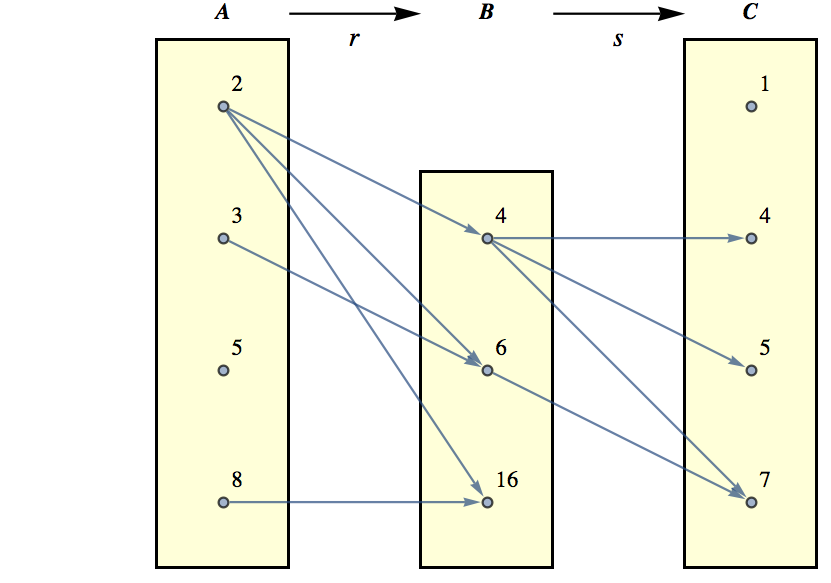
\includegraphics[width=1\linewidth]{images/graph-6-1-relation-composition.png}
\caption{Relation Composition - a graphical view\label{graph-6-1-relation-composition}}
\end{figure}
\par
Based on this observation, we can define a new relation, call it \(rs\), from \(A\) into \(C\). In order for \((a, c)\)
to be in \(rs\), it must be possible to travel along a path in Figure 6.1.2 from \(a\) to \(c\). In other words, \((a, c) \in rs\) if and only if \((\exists b)_B(a r b \textrm{ and } b s c)\). The name \(rs\) was chosen because it reminds us that this new relation was formed by the two previous relations \(r\) and \(s\). The complete listing of all elements in \(rs\) is \(\{(2, 4), (2, 5), (2, 7), (3, 7)\}\). We summarize in a definition.%
\begin{definition}[Composition of Relations]\label{def-composition-of-relations}
\index{Composition of Relations}\label{notation-3}
Let \(r\) be a relation from a set \(A\) into a set \(B\), and let \(s\) be a relation from \(B\) into a set \(C\). The composition of \(r\) with \(s\), written \(rs\), is the set of pairs of the form \((a, c) \in A\times C\), where \((a, c) \in rs\) if and only if there exists \(b \in B\) such that \((a, b) \in r\) and \((b, c) \in s\).%
\end{definition}
\par
Remark: A word of warning to those readers familiar with composition of functions. (For those who are not, disregard this remark. It will be repeated at an appropriate place in the next chapter.) As indicated above, the traditional way of describing a composition of two relations is \(rs\) where \(r\) is the first relation and \(s\) the second. However, function composition is traditionally expressed in the opposite order; that is, \(s\circ r\), where \(r\) is the first function and \(s\) is the second.%
\typeout{************************************************}
\typeout{Exercises 1.1.1 Exercises}
\typeout{************************************************}
\subsection[Exercises]{Exercises}\label{exercises-6-1}
\hypertarget{exercisegroup-1}{}\typeout{************************************************}
\typeout{Introduction  }
\typeout{************************************************}
A Exercises%
\begin{exercisegroup}
\item[1.]\hypertarget{exercise-1}{} For each of the following relations \(r\) defined on \(\mathbb{P}\), determine which of the given ordered pairs belong to \(r\)%
\par
\leavevmode%
\begin{enumerate}[label=\alph*]
\item\hypertarget{li-1}{} \(x r y\) iff \(x|y\);  (2, 3), (2, 4), (2, 8), (2, 17)%
\item\hypertarget{li-2}{} \(x r y\) iff \(x \leq  y\); (2, 3), (3, 2), (2, 4), (5, 8)%
\item\hypertarget{li-3}{} \(x r y\) iff \(y =x^2\) ; (1,1), (2, 3), (2, 4), (2, 6)%
\end{enumerate}
%
\par\smallskip
\par\smallskip
\noindent\textbf{Answer.}\hypertarget{answer-1}{}\quad
\leavevmode%
\begin{enumerate}[label=\alph*]
\item\hypertarget{li-4}{} \((2,4), (2,8)\)   %
\item\hypertarget{li-5}{} \((2, 3), (2, 4), (5,8)\)   %
\item\hypertarget{li-6}{} \((1,1), (2,4)\)%
\end{enumerate}
%
\item[2.]\hypertarget{exercise-2}{} The following relations are on \(\{\{1, 3, 5\}\}\). Let \(r\) be the relation \(x r y\) iff \(y = x + 2\) and \(s\) the
relation \(x s y\) iff \(x \leq  y\).%
\par
\leavevmode%
\begin{enumerate}[label=\alph*]
\item\hypertarget{li-7}{} List all elements in  \(rs\).%
\item\hypertarget{li-8}{} List all elements in  \(sr\).%
\item\hypertarget{li-9}{} Illustrate \(rs\) and \(sr\) via a diagram.%
\item\hypertarget{li-10}{} Is the relation (set) \(rs\) equal to the relation \(sr\)? Why?%
\end{enumerate}
%
\par\smallskip
\item[3.]\hypertarget{exercise-3}{} Let \(A = \{1,2,3,4,5\}\) and define \(r\) on A by \(x r y\) iff \(x + 1 = y\). We
define \(r^2 = r r\) and \(r^3 = r^2 r\). Find:%
\par
\leavevmode%
\begin{enumerate}[label=\alph*]
\item\hypertarget{li-11}{} \(r\)%
\item\hypertarget{li-12}{} \(r^2\)%
\item\hypertarget{li-13}{} \(r^3\)%
\end{enumerate}
%
\par\smallskip
\par\smallskip
\noindent\textbf{Answer.}\hypertarget{answer-2}{}\quad
\leavevmode%
\begin{enumerate}[label=\alph*]
\item\hypertarget{li-14}{} \(r=\{(1,2), (2,3), (3,4), (4,5)\}\)%
\item\hypertarget{li-15}{} \(r^2 = \{(1,3), (2,4), (3,5)\}=\{(x,y) : y=x+2, x,y\in A\}\)%
\item\hypertarget{li-16}{} \(r^3=\{(1,4), (2,5)\}=\{(x,y) : y=x+3, x,y \in  A\}\) %
\end{enumerate}
%
\item[4.]\hypertarget{exercise-4}{} Given \(s\) and \(t\), relations on \(\mathbb{Z}\),\( s = \{(1, n) : n \in \mathbb{Z}\}\) and \(t= \{(n, 1) : n \in  \mathbb{Z}\}\),
what are \(st\) and \(ts\)? Hint: Even when a relation involves infinite sets, you can often get insights into them by drawing
partial graphs.%
\par\smallskip
\end{exercisegroup}
\par\smallskip\noindent
\hypertarget{exercisegroup-2}{}\typeout{************************************************}
\typeout{Introduction  }
\typeout{************************************************}
B Exercises%
\begin{exercisegroup}
\item[5.]\hypertarget{exercise-5}{} Let \(\rho\) be the relation on the power set, \(\mathcal{P}(S )\), of a finite set S of cardinality \(n\). Define \(\rho\) by \((A,B)
\in \rho\) iff \(A\cap  B = \emptyset\).%
\par
\leavevmode%
\begin{enumerate}[label=\alph*]
\item\hypertarget{li-17}{} Consider the specific case \(n = 3\), and determine the cardinality of the set \(\rho\).%
\item\hypertarget{li-18}{} What is the cardinality of \(\rho\) for an arbitrary \(n\)? Express your answer in terms of \(n\). (Hint: There are three places that each element of S can go in building an element of \(\rho\).)%
\end{enumerate}
%
\par\smallskip
\par\smallskip
\noindent\textbf{Answer.}\hypertarget{answer-3}{}\quad
\leavevmode%
\begin{enumerate}[label=\alph*]
\item\hypertarget{li-19}{} When \(n=3\), there are 27 pairs in the relation.%
\item\hypertarget{li-20}{} Imagine building a pair of disjoint subsets of \(S\). For each element of \(S\) there are three places that it can go: into the first set of the ordered pair, into the second set, or into neither set. Therefore the number of pairs in the relation is \(3^n\), by the product rule.%
\end{enumerate}
%
\item[6.]\hypertarget{exercise-6}{} Let \(r_1\), \(r_2\), and \(r_3\) be relations on any set \(A\). Prove that if \(r_1\subseteq r_2\)then \(r_1r_3\subseteq r_2r_3\).%
\par\smallskip
\end{exercisegroup}
\par\smallskip\noindent
\typeout{************************************************}
\typeout{Section 1.2 Graphs of Relations on a Set}
\typeout{************************************************}
\section[Graphs of Relations on a Set]{Graphs of Relations on a Set}\label{s-graphs-of-relations-on-a-set}
In this section we introduce directed graphs as a way to visualize relations on a set. %
\par
Let \(A = \{0, 1,2,3\}\), and let  \[r = \{(0, 0), (0, 3), (1, 2), (2, 1), (3, 2), (2, 0)\}\]
In representing this relation as a graph, elements of \(A\) are called the vertices of the graph. They are typically represented by labeled points or small circles. We connect vertex \(a\) to vertex \(b\) with an arrow, called an edge, going from vertex \(a\) to vertex \(b\) if and only if \(a r b\).  This type of graph of a relation \(r\) is called a \terminology{directed graph} or \terminology{digraph}. \hyperref[fig-graph-6-2-1]{Figure~\ref{fig-graph-6-2-1}} is a digraph for \(r\). Notice that since 0 is related to itself, we draw a ``self-loop'' at 0.\index{Directed graph}\index{Digraph}%
\leavevmode%
\begin{figure}
\centering
\IfFileExists{images/graph-6-2-1.pdf}%
{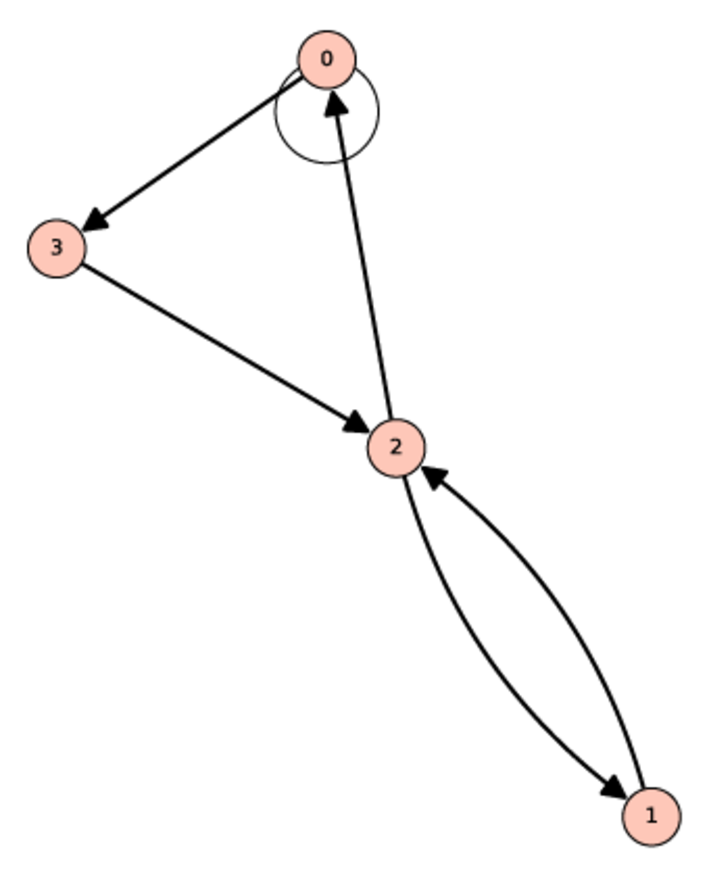
\includegraphics[width=1\linewidth]{images/graph-6-2-1.pdf}}%
{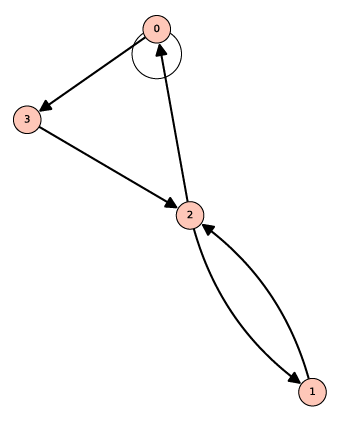
\includegraphics[width=1\linewidth]{images/graph-6-2-1.png}}
\caption{Digraph of a relation \label{fig-graph-6-2-1}}
\end{figure}
\par
The actual location of the vertices in a digraph is immaterial. The actual location of vertices we choose is called an \terminology{embedding of a graph}\index{Embedding of a graph}. The main idea is to place the vertices in such a way that the graph is easy to read. After drawing a rough-draft graph of a relation, we may decide to relocate the vertices so that the final result will be neater. \hyperref[fig-graph-6-2-1]{Figure~\ref{fig-graph-6-2-1}} could also
be presented as in \hyperref[fig-graph-6-2-2]{Figure~\ref{fig-graph-6-2-2}}.%
\leavevmode%
\begin{figure}
\centering
\IfFileExists{images/graph-6-2-2.pdf}%
{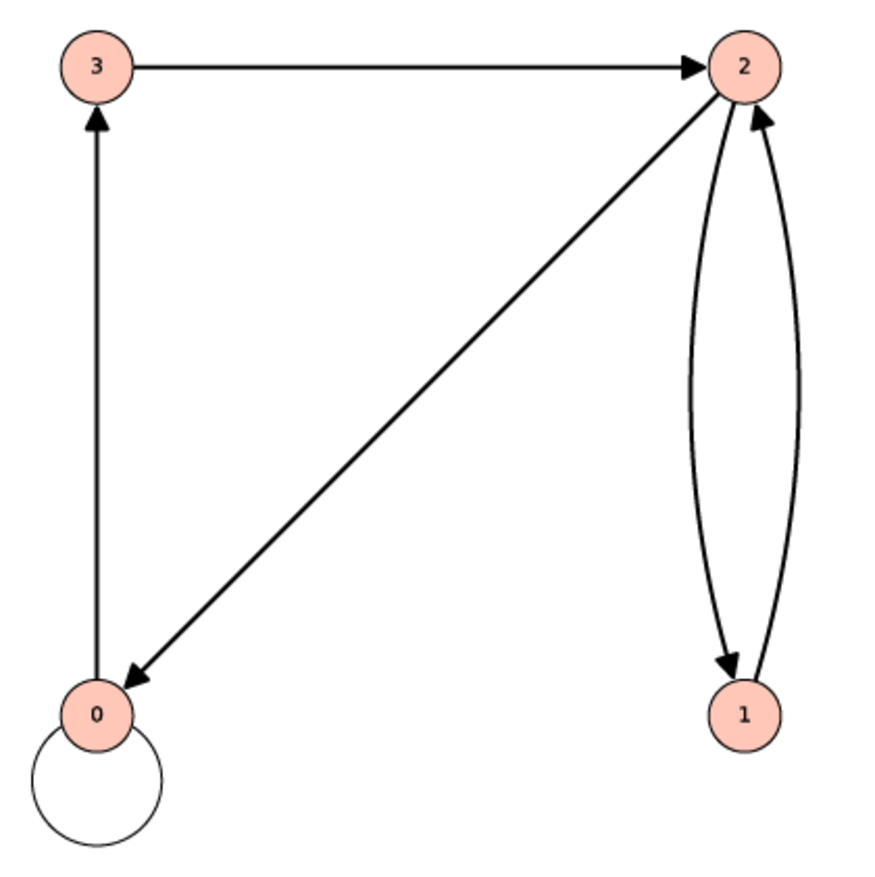
\includegraphics[width=1\linewidth]{images/graph-6-2-2.pdf}}%
{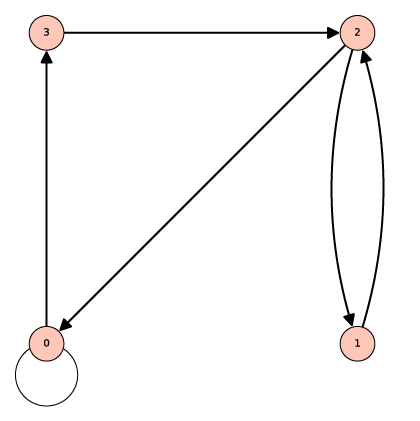
\includegraphics[width=1\linewidth]{images/graph-6-2-2.png}}
\caption{Alternate embedding of of the previous directed graph\label{fig-graph-6-2-2}}
\end{figure}
\par
A vertex of a graph is also called a node, point, or a junction. An edge of a graph is also referred to as an arc, a line, or a branch. Do not be concerned if two graphs of a given relation look different as long as the connections between vertices are are the same in two graphs.%
\begin{example}[Another directed graph.]\label{ex-another-simple-graph}
Consider the relation \(s\) whose digraph is \hyperref[fig-graph-6-2-3]{Figure~\ref{fig-graph-6-2-3}}. What information does this give us? The graph tells us that \(s\) is a relation on \(A = \{1, 2, 3\}\) and that \(s = \{(1, 2), (2, 1), (1, 3), (3, 1), (2, 3), (3, 3)\}\),%
\leavevmode%
\begin{figure}
\centering
\IfFileExists{images/graph-6-2-3.pdf}%
{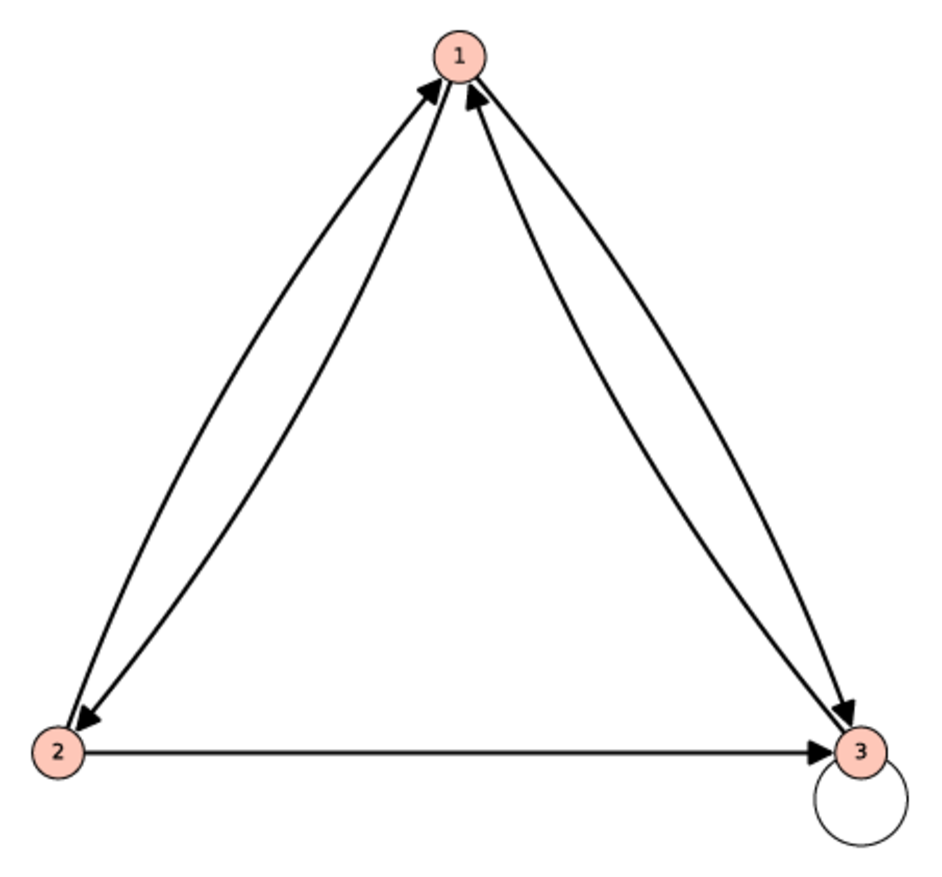
\includegraphics[width=1\linewidth]{images/graph-6-2-3.pdf}}%
{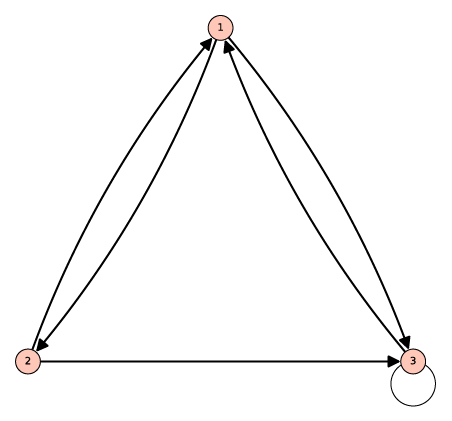
\includegraphics[width=1\linewidth]{images/graph-6-2-3.png}}
\caption{Digraph of the relation \(s\)\label{fig-graph-6-2-3}}
\end{figure}
\end{example}
\begin{example}[Ordering subsets of a two element universe]\label{ex-subsets-2-ordering}
 Let \(B = \{1,2\}\), and let \(A = \mathcal{P}(B) = \{0, \{1\}, \{2\}, \{1,2\}\}\). Then \(\subseteq\) is a relation on \(A\) whose digraph is \hyperref[fig-graph-6-2-subsets-2]{Figure~\ref{fig-graph-6-2-subsets-2}}.%
\leavevmode%
\begin{figure}
\centering
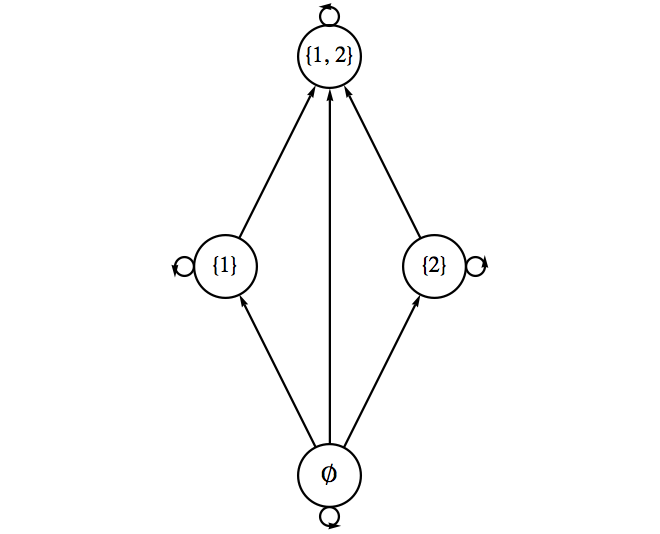
\includegraphics[width=1\linewidth]{images/graph-6-2-subsets-2.png}
\caption{Graph for set containment on subsets of \(\{1,2\}\) \label{fig-graph-6-2-subsets-2}}
\end{figure}
\par
We will see in the next section that since \(\subseteq\) has certain structural properties that describe ``partial orderings.'' We will be able to draw a much simpler type graph than this one, but for now the graph above serves our purposes.%
\end{example}
\typeout{************************************************}
\typeout{Exercises 1.2.1 Exercises}
\typeout{************************************************}
\subsection[Exercises]{Exercises}\label{exercises-6-2}
\hypertarget{exercisegroup-3}{}\typeout{************************************************}
\typeout{Introduction  }
\typeout{************************************************}
A Exercises%
\begin{exercisegroup}
\item[1.]\hypertarget{exercise-7}{} Let \(A = \{1, 2, 3, 4\}\), and let \(r\) be the relation \(\leq\) on \(A\) Draw a digraph for \(r\).%
\par\smallskip
\par\smallskip
\noindent\textbf{Answer.}\hypertarget{answer-4}{}\quad
\leavevmode%
\begin{figure}
\centering
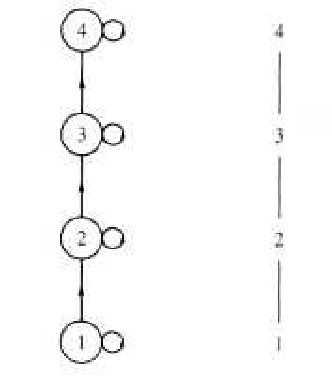
\includegraphics[width=1\linewidth]{images/fig-sol-6-2-1.png}
\end{figure}
\item[2.]\hypertarget{exercise-8}{} Let \(B = \{1,2, 3, 4, 6, 8, 12, 24\}\), and let \(s\) be the relation ``divides,'' on \(B\). Draw a digraph for \(s\). %
\par\smallskip
\item[3.]\hypertarget{exercise-9}{}  Let \(A=\{1,2,3,4,5\}\). Define \(t\) on \(A\) by \(a t b\) if and only if \(b - a\) is even. Draw a digraph for \(t\).%
\par\smallskip
\par\smallskip
\noindent\textbf{Answer.}\hypertarget{answer-5}{}\quad
 See Figure 13.1.1 of Section 13.1.%
\item[4.]\hypertarget{exercise-10}{}\leavevmode%
\begin{enumerate}[label=\alph*]
\item\hypertarget{li-21}{}Let \(A\) be the set of strings of 0's and 1's of length 3 or less. Define the relation of \(d\) on A by \(x d y\) if \(x\) is contained within \(y\). For example, \(01 d 101\). Draw a digraph for this relation. %
\item\hypertarget{li-22}{} Do the same for the relation \(p\) defined by \(x p y\) if \(x\) is a prefix of \(y\). For example, \(10 p 101\), but \(01 p 101\) is false.%
\end{enumerate}
%
\par\smallskip
\end{exercisegroup}
\par\smallskip\noindent
\hypertarget{exercisegroup-4}{}\typeout{************************************************}
\typeout{Introduction  }
\typeout{************************************************}
B Exercises%
\begin{exercisegroup}
\item[5.]\hypertarget{exercise-11}{} Recall the relation in Exercise 5 of Section 6.1, \(\rho\) defined on the power set, \(\mathcal{P}(S)\), of a set \(S\). The definition
was \((A,B) \in \rho\) iff \(A\cap  B = \emptyset\). Draw the digraph for \(\rho\) where \(S = \{a, b\}\). %
\par\smallskip
\par\smallskip
\noindent\textbf{Answer.}\hypertarget{answer-6}{}\quad
 A Hasse diagram cannot be used because not every set is related to itself. Also, \(\{a\}\) and \(\{b\}\) are related in both directions.
%
\item[6.]\hypertarget{exercise-12}{} Let \(C= \{1,2, 3, 4, 6, 8, 12, 24\}\) and define \(t\) on \(C\) by
\(a t b\) if and only if \(a\) and \(b\) share a common divisor greater than 1.  Draw a digraph for \(t\).%
\par\smallskip
\end{exercisegroup}
\par\smallskip\noindent
\typeout{************************************************}
\typeout{Section 1.3 Properties of Relations}
\typeout{************************************************}
\section[Properties of Relations]{Properties of Relations}\label{s-properties-of-relations}
\typeout{************************************************}
\typeout{Subsection 1.3.1 Individual Properties}
\typeout{************************************************}
\subsection[Individual Properties]{Individual Properties}\label{ss-individual-properties}
Consider the set \(B = \{1, 2, 3, 4, 6, 12, 36, 48\}\) and the relations ``divides'' and \(\leq \) on \(B\). We notice that these two relations on \(B\) have three properties in common:%
\par
\leavevmode%
\begin{itemize}[label=\textbullet]
\item{}Every element in \(B\) divides itself and is less than or equal to itself. This is called the reflexive property.%
\item{}If we search for two elements from \(B\) where the first divides the second and the second divides the first, then we are forced to choose the the two numbers to be the same. In other words, no two \emph{different} numbers are related in both directions. The reader can verify that a similar fact is true for the relation \(\leq \) on \(B\). This is called the antisymmetric property.%
\item{}Next if we choose three numbers from \(B\) such that the first divides the second and the second divides the third, then we always find that the first number to divides the third.  Again, the same is true if we replace ``divides'' with ``is less than or equal to.'' This is called the transitive property.%
\end{itemize}
%
\par
Relations that satisfy these properties are of special interest to us. Formal definitions of the properties follow.%
\begin{definition}[Reflexive Relation]\label{def-reflexive-relation}
\index{Reflexive Relation}Let \(A\) be a set and let \(r\) be a relation on \(A\).
r is \terminology{reflexive} if and only if \(a r a\) for all \(a \in A\).%
\end{definition}
\begin{definition}[Antisymmetric Relation]\label{def-antisymmetric-relation}
\index{Antisymmetric Relation}Let \(A\) be a set and let \(r\) be a relation on \(A\).  Then \(r\) is \terminology{antisymmetric} if and only if whenever \(a r b\) and \(a \neq  b\) then \(b r a\) is false.%
\end{definition}
\par
An equivalent condition for antisymmetry is that if \(a r b\) and  \(b r a\) then \(a = b\). You are encouraged to convince yourself that this is true.  This condition is often more convenient to prove than the definition, even thought the definition is probably easier to understand.%
\par
A word of warning about antisymmetry: Students frequently find it difficult to understand this definition. Keep in mind that this term is defined through an ``If . .. then . . .'' statement. The question that you must ask is: Is it true that whenever there are elements \(a\) and \(b\) from \(A\) where \(a r b\) and \(a \neq  b\), it follows that \(b\) is not related to \(a\)? If so, then the relation  is antisymmetric.%
\par
Another way to determine whether a relation is antisymmetric is to examine (or imagine) its digraph. The relation is not antisymmetric if there exists a pair of vertices that are connected by edges in both directions.%
\begin{definition}[Transitive Relation]\label{def-transitive-relation}
\index{Transitive Relation}Let \(A\) be a set and let \(r\) be a relation on \(A\).
r is \terminology{transitive} if and only if whenever \(a r b\) and \(b r c\) then \(a r c\).%
\end{definition}
\typeout{************************************************}
\typeout{Subsection 1.3.2 Partial Orderings}
\typeout{************************************************}
\subsection[Partial Orderings]{Partial Orderings}\label{ss-partial-ordering}
Not all relations have all three of the properties discussed above, but those that do are a special type of relation.%
\begin{definition}[Partial Ordering]\label{partial-ordering}
\index{Partial Ordering}A relation on a set \(A\) that is reflexive, antisymmetric, and transitive is called a partial ordering on \(A\). A set on which there is a partial ordering relation defined is called a \terminology{partially ordered set}\index{Partially ordered set} or \terminology{poset}\index{Poset}.%
\end{definition}
\begin{example}[Set Containment as a Partial Ordering]\label{ex-subset-partial-ordering}
Let \(A\) be a set. Then \(\mathcal{P}(A)\) together with the relation \(\subseteq\) (set containment) is a poset.
To prove this we observe that the three properties hold, as discussed in Chapter 4.%
\par
\leavevmode%
\begin{itemize}[label=\textbullet]
\item{}Let \(B \in  \mathcal{P}(A)\). The fact that \(B \subseteq  B\) follows from the definition of subset. Hence, set containment is reflexive.%
\item{}Let \(B_1, B_2 \in \mathcal{P}(A)\) and assume that \(B_1\subseteq  B_2\) and \(B_1\neq  B_2\) . Could it be that \(B_2\subseteq  B_1\)? No.
There must be some element \(a\in A\) such that \(a \notin B_1\), but \(a\in B_2\). This is exactly what we need to conclude that \(B_2\) is not contained in \(B_1\).  Hence, set containment is antisymmetric.%
\item{}Let \(B_1, B_2,B_3 \in \mathcal{P}(A)\) and assume that \(B_1 \subseteq  B_2\) and \(B_2 \subseteq  B_3\) . Does it follow that \(B_1 \subseteq B_3\) ? Yes, if \(a\in B_1\), then \(a\in B_2\) because \(B_1 \subseteq  B_2\). Now that we have \(a\in B_2\) and we have assumed \(B_2 \subseteq B_3\), we conclude that \(a\in B_3\).  Therefore, \(B_1\subseteq B_3\) and so set containment is transitive.%
\end{itemize}
%
\par
\hyperref[fig-graph-6-2-subsets-2]{Figure~\ref{fig-graph-6-2-subsets-2}} is the graph for the ``set containment'' relation on \(\{1,2\}\).%
\end{example}
\par
\hyperref[fig-graph-6-2-subsets-2]{Figure~\ref{fig-graph-6-2-subsets-2}} is helpful insofar as it reminds us that each set is a subset of itself and shows us at a glance the relationship between the various subsets in \(\mathcal{P} (\{1,2\})\). However, when a relation is a partial ordering, we can streamline a graph like this one.  The streamlined
form of a graph is called a \terminology{Hasse diagram} or \terminology{ordering diagram}.  A Hasse diagram takes into account the following facts.%
\par
\leavevmode%
\begin{itemize}[label=\textbullet]
\item{} By the reflexive property, each vertex must be related to itself, so the arrows from a vertex to itself (called ``self-loops'') are
not drawn in a Hasse diagram. They are simply assumed.%
\item{}  By the antisymmetry property, connections between two distinct elements in a directed graph can only go one way, if at all.  When there
is a connection, we agree to always place the second element above the first (as we do above with the connection from \(\{1\}\) to \(\{1,2\}\)).
For this reason, we can just draw a connection without an arrow, just a line.%
\item{} By the transitive property, if there are edges connecting one element up to a second element and the second element up to a third element,
then there will be a direct connection from the first to the third. We see this in \hyperref[fig-graph-6-2-subsets-2]{Figure~\ref{fig-graph-6-2-subsets-2}} with \(\emptyset\) connected to \(\{1\}\)\(\)and
then \(\{1\}\) connected to \(\{1,2\}\). Notice the edge connecting \(\emptyset\) to \(\{1,2\}\).  Whenever we identify this situation, remove
the connection from the first to the third in a Hasse diagram and simply observe that an upward path of any length implies that the lower element
is related to the upper one.
%
\end{itemize}
%
\par
Using these observations as a guide, we can draw a Hasse diagram for \(\subseteq\) on \(\{1,2\}\) as in Figure 6.3.2.%
\leavevmode%
\begin{figure}
\centering
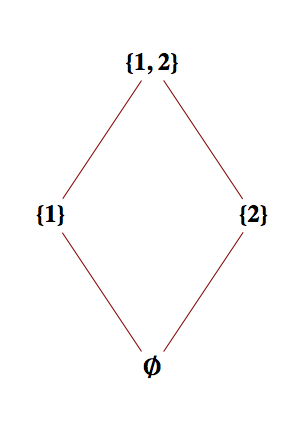
\includegraphics[width=1\linewidth]{images/subsets_2_hasse.png}
\caption{Hasse diagram for set containment on subsets of \(\{1,2\}\)
                \label{subsets_2_hasse}}
\end{figure}
\begin{example}[Definition of a relation using a Hasse diagram]\label{ex-def-by-hasse}
Consider the partial ordering relation \(s\) whose Hasse diagram is \hyperref[fig-pentagonal-hasse]{Figure~\ref{fig-pentagonal-hasse}}.%
\leavevmode%
\begin{figure}
\centering
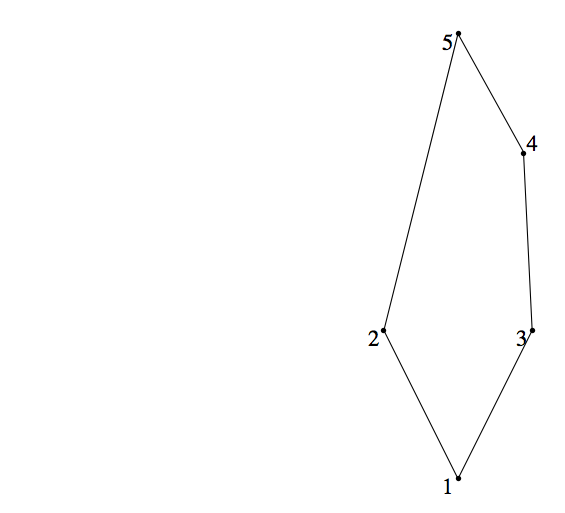
\includegraphics[width=1\linewidth]{images/pentagonal-hasse.png}
\caption{Hasse diagram for for the pentagonal poset
                \label{fig-pentagonal-hasse}}
\end{figure}
\par
How do we read this diagram? What is \(A\)? What is \(s\)? What does the digraph of s look like? Certainly \(A = \{1,2,3,4,5\}\) and
\(1 s 2\), \(3 s 4\), \(1 s 4\), \(1 s 5\), etc., Notice that \(1 s 5\) is implied by the fact that there is a path of length three upward
from 1 to 5. This follows from the edges that are shown and the transitive property that is presumed in a poset.  Since \(1 s 3\) and \(3 s
4\), we know that \(1 s 4\). We then combine \(1 s 4\) with \(4 s 5\) to infer \(1 s 5\).  Without going into details why, here is
a complete list of pairs defined by \(s\).
\[s = \{(1,1),(2,2),(3,3),(4,4),(5,5),(1,3),(1,4),(1,5),(1,2),(3,4),(3,5),(4,5),(2,5)\}\]%
\par
A digraph for \(s\) is \hyperref[fig-pentagonal-digraph]{Figure~\ref{fig-pentagonal-digraph}}. It is certainly more complicated to read and difficult to draw than the Hasse diagram.%
\leavevmode%
\begin{figure}
\centering
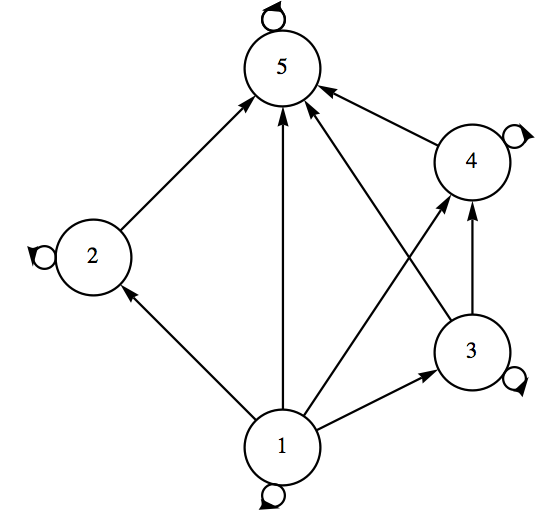
\includegraphics[width=1\linewidth]{images/pentagonal-digraph.png}
\caption{Digraph for for the pentagonal poset
                \label{fig-pentagonal-digraph}}
\end{figure}
\end{example}
\par
A classic example of a partial ordering relation is \(\leq \) on the real numbers, \(\mathbb{R}\). Indeed, when graphing partial ordering relations,
it is natural to ``plot'' the elements from the given poset starting with the ``least'' element to the ``greatest'' and to use terms
like ``least,'' ``greatest,'' etc. Because of this the reader should be forewarned that some texts use the symbol \(\leq\) for arbitrary
partial orderings. This can be quite confusing for the novice, so we continue to use generic letters \(r\), \(s\), etc.
%
\typeout{************************************************}
\typeout{Subsection 1.3.3 Equivalence Relations}
\typeout{************************************************}
\subsection[Equivalence Relations]{Equivalence Relations}\label{ss-equivalence-relations}
\index{Equivalence Relations}Another common property of relations is symmetry.%
\begin{definition}[Symmetric Relation]\label{def-symmetric-relation}
\index{Symmetric 
Relation}Let \(r\) be a relation on a set \(A\). \(r\) is \terminology{symmetric} if and only if whenever \(a r b\), it follows that \(b r a\).%
\end{definition}
\par
Consider the relation of equality defined on any set \(A\). Certainly \(a = b\) implies that\(b = a\) so equality is a symmetric relation on \(A\).%
\par
Surprisingly, equality is also an antisymmetric relation on \(A\). This is due to the fact that the condition that defines the antisymmetry property, \(a = b\) and \(a \neq  b\), is a contradiction. Remember, a conditional proposition is always true when the condition is false. So a relation can be both symmetric and antisymmetric on a set! Again recall that these terms are \emph{not} negatives of one other. That said, there are very few important relations other than equality that are both symmetric and antisymmetric.%
\begin{definition}[Equivalence Relation]\label{def-equivalence-relation}
\index{Equivalence Relation}A relation \(r\) on a set \(A\) is called an equivalence relation if and only if it is reflexive, symmetric, and transitive.%
\end{definition}
\par
The classic example of an equivalence relation is equality on a set \(A\). In fact, the term equivalence relation is used because those relations which satisfy the definition behave quite like the equality relation. Here is another important equivalence relation.%
\begin{example}[Equivalent Fractions]\label{ex-fraction-equivalence}
Let \(\mathbb{Z}\)* be the set of nonzero integers. One of the most basic equivalence relations in mathematics is the relation \(q\) on \(\mathbb{Z}\times \mathbb{Z}^*\) defined by \((a, b) q(c, d)\) if and only if \(a d = b c\). We will leave it to the reader to, verify
that \(q\) is indeed an equivalence relation. Be aware that since the elements of \(\mathbb{Z}\times \mathbb{Z}^*\) are ordered pairs, proving symmetry involves four numbers and transitivity involves six numbers. Two ordered pairs, \((a, b)\) and \((c, d)\), are related if the fractions \(\frac{a}{b}\) and \(\frac{c}{d}\) are numerically equal.
%
\end{example}
\par
Our next example involves the following fundamental relations on the set of integers.%
\begin{definition}[Congruence Modulo \(m\)]\label{def-congruence-mod-m}
\index{Congruence Modulo m}\label{notation-4}
Let \(m\) be a positive integer, \(m\geq 2\).  We define \terminology{congruence modulo m} to be the relation \(\equiv_m\) defined on the integers by 
	\[a \equiv_m b \Leftrightarrow m \mid (a-b)\]
%
\end{definition}
\par
We observe the following about congurence modulo \(m\):%
\par
\leavevmode%
\begin{itemize}[label=\textbullet]
\item{}This relation is reflexive, for if \(a \in  \mathbb{Z} \),  \(m \mid (a-a) \Rightarrow  a\equiv_ma \).%
\item{}This relation is symmetric. We can prove this through the following chain of implications. 
\begin{equation*}
\begin{split}
a \equiv_m b &\Rightarrow   m \mid (a-b)\\
   & \Rightarrow \textrm{For  some } k \in \mathbb{Z}, a-b = m k \\
	& \Rightarrow b-a = m (-k)\\
	& \Rightarrow  m \mid (b-a)\\
	& \Rightarrow b \equiv_m a 
\end{split}
\end{equation*}%
\item{} Finally, this relation is transitive.  We leave it to the reader to prove that if \(a \equiv _mb \) and \(b\equiv _mc\), then \(a \equiv _mc\).%
\end{itemize}
%
\par
Frequently, you will see the equivalent notation \(a \equiv b (\textrm{mod } m)\) for congruence modulo \(m\).%
\begin{example}[Random Relations usually have no properties]\label{ex-no-propery-relation}
Consider the relation s described by the digraph in \hyperref[fig-graph-6-3-5]{Figure~\ref{fig-graph-6-3-5}}. This was created by randomly selecting whether or not two elements from \(\{a,b,c\}\) were related or not. %
\par
\leavevmode%
\begin{itemize}[label=\textbullet]
\item{}This relation is not reflexive, Why?%
\item{}It is not antisymmetric, Why?%
\item{}Also, it is not symmetric, Why?%
\item{}It is not transitive, Why?%
\item{}Is \(s\) an equivalence relation or a partial ordering? %
\end{itemize}
%
\leavevmode%
\begin{figure}
\centering
\IfFileExists{images/graph-6-3-5.pdf}%
{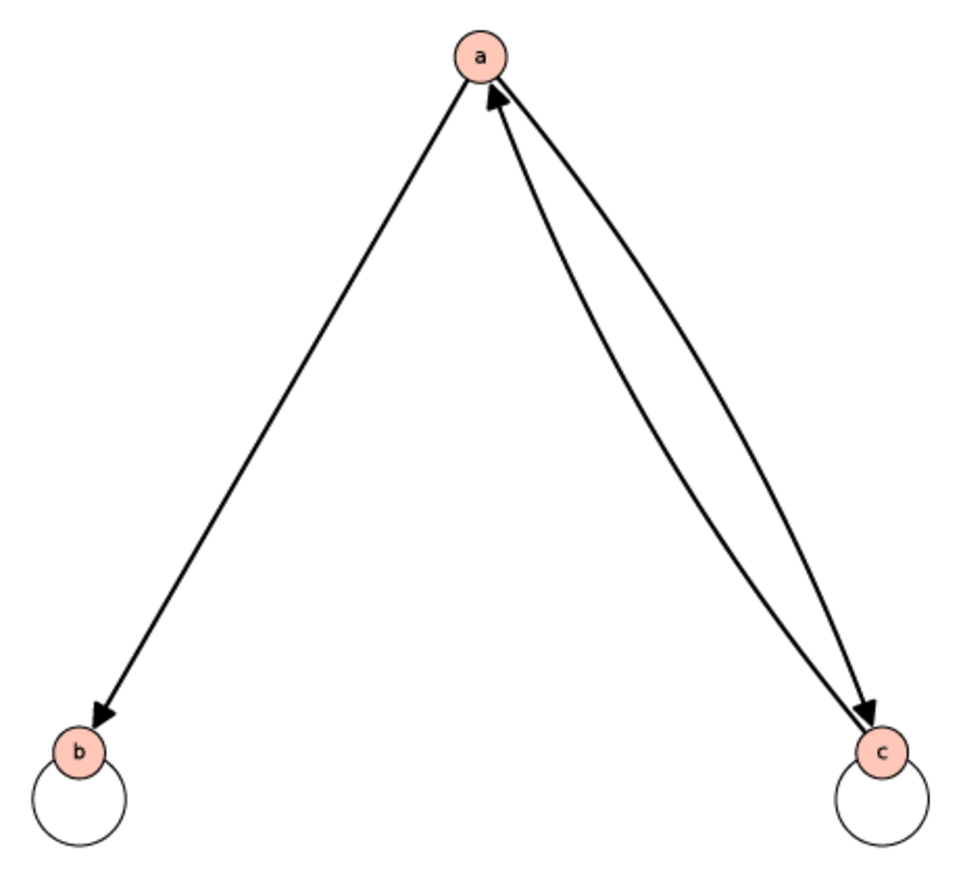
\includegraphics[width=1\linewidth]{images/graph-6-3-5.pdf}}%
{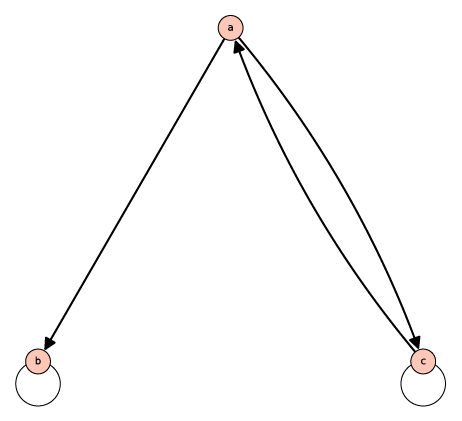
\includegraphics[width=1\linewidth]{images/graph-6-3-5.png}}
\caption{Digraph of a random relation \(r\)\label{fig-graph-6-3-5}}
\end{figure}
\par
Not every random choice of a relation will be so totally negative, but as the underlying set increases, the likelihood any of the properties are true begins to vanish.%
\end{example}
\typeout{************************************************}
\typeout{Exercises 1.3.4 Exercises}
\typeout{************************************************}
\subsection[Exercises]{Exercises}\label{exercises-6-3}
\hypertarget{exercisegroup-5}{}\typeout{************************************************}
\typeout{Introduction  }
\typeout{************************************************}
A Exercises%
\begin{exercisegroup}
\item[1.]\hypertarget{exercise-13}{}\leavevmode%
\begin{enumerate}[label=\alph*]
\item\hypertarget{li-40}{}Let \(B = \{a, b\}\) and \(U = \mathcal{P}(B)\). Draw a Hasse diagram for \(\subseteq \) on \(U\).%
\item\hypertarget{li-41}{}Let \(A = \{1,2, 3, 6\}\). Show that divides, \(\mid \), is a partial ordering on \(A\). %
\item\hypertarget{li-42}{}Draw a Hasse diagram for divides on \(A\).%
\item\hypertarget{li-43}{}Compare the graphs of parts a and c.%
\end{enumerate}
%
\par\smallskip
\par\smallskip
\noindent\textbf{Answer.}\hypertarget{answer-7}{}\quad
\leavevmode%
\begin{enumerate}[label=\alph*]
\item\hypertarget{li-44}{}\leavevmode%
\begin{figure}
\centering
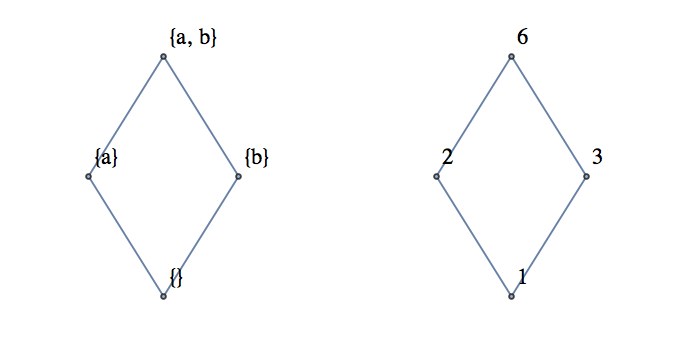
\includegraphics[width=1\linewidth]{images/fig-sol-6-3-1.png}
\end{figure}
%
\item\hypertarget{li-45}{} The graphs are the same if we disregard the names of the vertices.%
\end{enumerate}
%
\item[2.]\hypertarget{exercise-14}{}Repeat Exercise 1 with \(B = \{a, b, c\}\) and \( A = \{1, 2, 3, 5, 6, 10, 15, 30\}\).
%
\par\smallskip
\item[3.]\hypertarget{exercise-15}{}\leavevmode%
\begin{enumerate}[label=\alph*]
\item\hypertarget{li-46}{}Consider the relations defined by the digraphs in \hyperref[fig-exercises-6-digraphs]{Figure~\ref{fig-exercises-6-digraphs}}. Determine whether the given relations are reflexive, symmetric, antisymmetric,
or transitive. Try to develop procedures for determining the validity of these properties from the graphs, %
\item\hypertarget{li-47}{}Which of the graphs are of equivalence relations or of partial orderings?%
\end{enumerate}
%
\leavevmode%
\begin{figure}
\centering
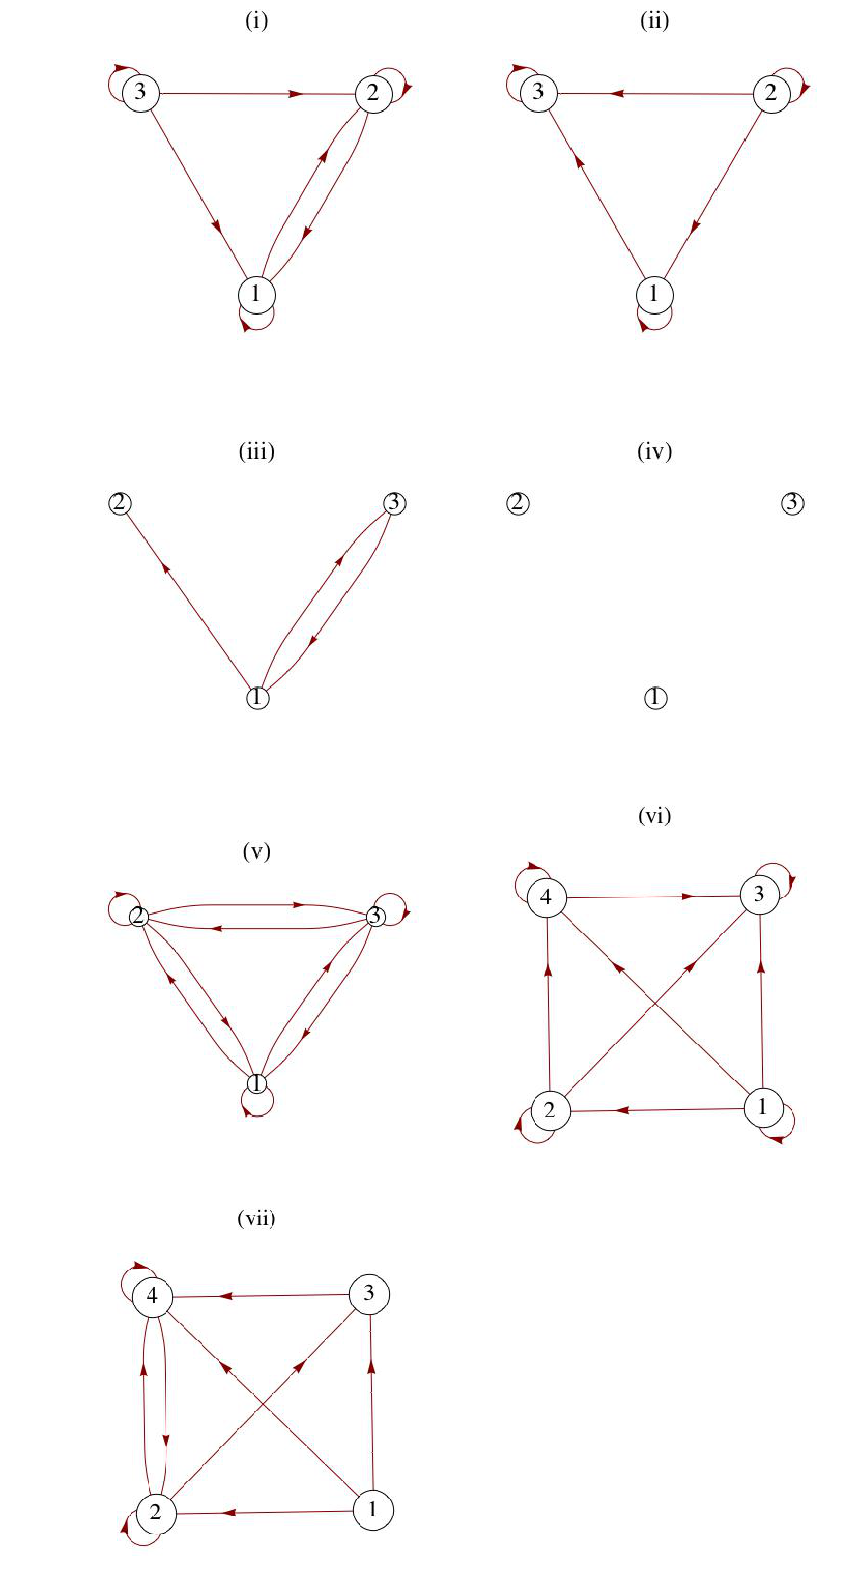
\includegraphics[width=1\linewidth]{images/exercises-6-digraphs.png}
\caption{Some digraphs of relations\label{fig-exercises-6-digraphs}}
\end{figure}
\par\smallskip
\par\smallskip
\noindent\textbf{Answer.}\hypertarget{answer-8}{}\quad
\leavevmode%
\begin{enumerate}[label=\roman*]
\item\hypertarget{li-48}{}\leavevmode%
\begin{table}
\centering
\begin{tabular}{lllll}
Part&reflexive?&symetric?&antisymmetric?&transitive?\tabularnewline[0pt]
i&yes&no&no&yes\tabularnewline[0pt]
ii&yes&no&yes&yes\tabularnewline[0pt]
iii&no&yes&no&yes\tabularnewline[0pt]
iv&no&yes&yes&yes\tabularnewline[0pt]
v&yes&yes&no&yes\tabularnewline[0pt]
vi&yes&no&yes&yes\tabularnewline[0pt]
vii&no&no&no&no
\end{tabular}
\end{table}
%
\item\hypertarget{li-49}{} Graphs ii and vi show partial ordering relations. Graph v is of an equivalence relation. %
\end{enumerate}
%
\item[4.]\hypertarget{exercise-16}{}Determine which of the following are equivalence relations and/or partial ordering relations for the given sets:%
\par
\leavevmode%
\begin{enumerate}[label=\alph*]
\item\hypertarget{li-50}{} \(A = \{\textrm{ lines in the plane}\}\): \(x r y\) if and only if \(x\) is parallel to \(y\).%
\item\hypertarget{li-51}{} \(A = \mathbb{R}\); \(x r y\) if and only if \(\lvert x -y \rvert \leq  7\).%
\end{enumerate}
%
\par\smallskip
\item[5.]\hypertarget{exercise-17}{}Consider the  relation on \(\{1, 2, 3, 4, 5, 6\}\) defined by  \(r = \{(i,j): \mid i - j\mid  = 2\}\).%
\par
\leavevmode%
\begin{enumerate}[label=\alph*]
\item\hypertarget{li-52}{} Is \(r\) reflexive?%
\item\hypertarget{li-53}{} Is \(r\) symmetric?%
\item\hypertarget{li-54}{} Is \(r\) transitive?%
\item\hypertarget{li-55}{} Draw a graph of \(r\).%
\end{enumerate}
%
\par\smallskip
\par\smallskip
\noindent\textbf{Answer.}\hypertarget{answer-9}{}\quad
\leavevmode%
\begin{enumerate}[label=\alph*]
\item\hypertarget{li-56}{} No, since \(\mid 1-1\mid =0\neq 2\), for example%
\item\hypertarget{li-57}{} Yes, because \(\mid i-j\mid =\)\(\mid j-i\mid \).%
\item\hypertarget{li-58}{} No, since \(\mid 2-4\mid =2\) and \(\mid 4-6\mid =2\), but \(\mid 2-6\mid =4\neq 2\), for example.%
\item\hypertarget{li-59}{}\leavevmode%
\begin{figure}
\centering

\includegraphics[width=1\linewidth]{images/fig-sol-6-3-5.png}
\end{figure}
%
\end{enumerate}
%
\item[6.]\hypertarget{exercise-18}{}For the set of cities on a map, consider the relation \(x r y\) if and only if city \(x\) is connected by a road to city \(y\). A city is considered to be connected to itself, and two cities are connected even though there are cities on the road between them. Is this an equivalence
relation or a partial ordering? Explain.%
\par\smallskip
\item[7.]\hypertarget{exercise-19}{} Let \(A = \{0, 1, 2, 3\}\) and let
\[r = \{(0, 0), (1, 1), (2, 2), (3, 3), (1, 2),(2, 1), (3, 2), (2, 3), (3, 1), (1, 3)\}\]%
\par
\leavevmode%
\begin{enumerate}[label=\alph*]
\item\hypertarget{li-60}{}Verify that \(r\) is an equivalence relation on \(A\).%
\item\hypertarget{li-61}{}Let \(a \in A\) and define \(c(a) = \{b \in A \mid a r b\}\)\label{notation-5}
. \(c(a)\) is called the \terminology{equivalence class of \(a\) under \(r\)}\index{Equivalence Class}. Find \(c(a)\) for each element \(a \in A\).%
\item\hypertarget{li-62}{}Show that \(\{c(a) \mid  a \in A\}\) forms a partition of A for this set A.%
\item\hypertarget{li-63}{}Let \(r\) be an equivalence relation on an arbitrary set \(A\). Prove that the set of all equivalence classes under \(r\) constitutes a partition of \(A\).
%
\end{enumerate}
%
\par\smallskip
\par\smallskip
\noindent\textbf{Answer.}\hypertarget{answer-10}{}\quad
\leavevmode%
\begin{enumerate}[label=\alph*]
\item\hypertarget{li-64}{}%
\item\hypertarget{li-65}{} \(c(0)=\{0\}, c(1)=\{1,2,3\}=c(2)=c(3)\)%
\item\hypertarget{li-66}{} \(c(0)\cup c(1)=A\) and \(c(0)\cap c(1)=\emptyset\)%
\item\hypertarget{li-67}{} Let \(A\) be any set and let \(r\) be an equivalence relation on \(A\). Let \(a\) be any element of \(A\). \(a\in c(a)\) since \(r\) is reflexive, so each element of \(A\) is in some equivalence class. Therefore, the union of all equivalence classes equals \(A\). Next we show that any two equivalence classes are either identical or disjoint and we are done. Let \(c(a)\) and \(c(b)\) be two equivalence classes, and assume that \(c(a)\cap c(b)\neq \emptyset\). We want to show that \(c(a)=c(b)\). To show that \(c(a)\subseteq c(b)\), let \(x\in c(a)\). \(x\in c(a) \Rightarrow a r x \). Also, there exists an element, \(y\), of \(A\) that is in the intersection of \(c(a)\)
and \(c(b)\) by our assumption. Therefore,
  \[
  \begin{split}
  a r y \land b r y &\Rightarrow  a r y \land y r b \quad r\textrm{  is symmetric}\\
			&\Rightarrow  a r b  \quad \textrm{ transitivity of }r \\
	\end{split}
	\]%
\par
 Next,
     \begin{equation*}
     \begin{split}
     a r x \land a r b &\Rightarrow x r a \land a r b\\
		&\Rightarrow  x r b\\
		&\Rightarrow  b r x\\
		& \Rightarrow  x \in c(b)\\
		\end{split}
		\end{equation*}
		%
\par
 Similarly, \(c(b)\subseteq c(a)\)  \(\square\) %
\end{enumerate}
%
\item[8.]\hypertarget{exercise-20}{}Define \(r\) on the power set of \(\{1, 2, 3\}\) by \(A r B \Leftrightarrow  \lvert A \rvert = \lvert B \rvert \). Prove that \(r\) is an equivalence
relation. What are the equivalence classes under \(r\)?%
\par\smallskip
\item[9.]\hypertarget{exercise-21}{}Consider the following relations on \(\mathbb{Z}_8= \{0, 1, . . . , 7\}\). Which are equivalence relations? For the equivalence relations, list the equivalence classes.%
\par
\leavevmode%
\begin{enumerate}[label=\alph*]
\item\hypertarget{li-68}{} \(a r b\) iff the English spellings of a and b begin with the same letter.%
\item\hypertarget{li-69}{} \(a s b\) iff \(a - b\) is a positive integer.%
\item\hypertarget{li-70}{} \(a t b\) iff \(a-b\) is an even integer.%
\end{enumerate}
%
\par\smallskip
\par\smallskip
\noindent\textbf{Answer.}\hypertarget{answer-11}{}\quad
\leavevmode%
\begin{enumerate}[label=\alph*]
\item\hypertarget{li-71}{}Equivalence Relation,
 \(c(0)=\{0\},c(1)=\{1\},c(2)=\{2,3\} =c(3),c(4)=\{4,5\}=c(5)\), and
 \(c(6)=\{6,7\}=c(7)\)%
\item\hypertarget{li-72}{}  Not an Equivalence Relation.%
\item\hypertarget{li-73}{}  Equivalence Relation,
 \(c(0)=\{0,2,4,6\}=c(2)=c(4)=c(6)\)  and 
 \(c(1)=\{1,3,5,7\}=c(3)=c(5)=c(7)\)%
\end{enumerate}
%
\item[10.]\hypertarget{exercise-22}{}\leavevmode%
\begin{enumerate}[label=\alph*]
\item\hypertarget{li-74}{}Prove that conguence modulo \(m\) is a transitive?%
\item\hypertarget{li-75}{}What are the equivalence classes under conguence modulo 2?%
\item\hypertarget{li-76}{} What are the equivalence classes under conguence modulo 10? %
\end{enumerate}
%
\par\smallskip
\end{exercisegroup}
\par\smallskip\noindent
\hypertarget{exercisegroup-6}{}\typeout{************************************************}
\typeout{Introduction  }
\typeout{************************************************}
B Exercises%
\begin{exercisegroup}
\item[11.]\hypertarget{exercise-23}{}In this exercise, we prove that implication is a partial ordering. Let \(A\) be any set of propositions.%
\par
\leavevmode%
\begin{enumerate}[label=\alph*]
\item\hypertarget{li-77}{} Verify that \(q \to  q\) is a tautology, thereby showing that \(\Rightarrow\) is a reflexive relation on \(A\).%
\item\hypertarget{li-78}{} Prove that \(\Rightarrow\) is antisymmetric on A. Note: we do not use = when speaking of propositions, but rather equivalence, \(\Leftrightarrow\).%
\item\hypertarget{li-79}{} Prove that \(\Rightarrow\) is transitive on \(A\).%
\item\hypertarget{li-80}{} Given that \(q_i\) is the proposition \(n < i\) on \(\mathbb{N}\), draw the Hasse diagram for the relation \(\Rightarrow\) on \(\{q_1, q_2, q_3,\ldots \}\).%
\end{enumerate}
%
\par\smallskip
\par\smallskip
\noindent\textbf{Answer.}\hypertarget{answer-12}{}\quad
\leavevmode%
\begin{enumerate}[label=\alph*]
\item\hypertarget{li-81}{}%
\item\hypertarget{li-82}{} The proof follows from the biconditional equivalence in Table 3.4.2.%
\item\hypertarget{li-83}{} Apply the chain rule.%
\item\hypertarget{li-84}{}\leavevmode%
\begin{figure}
\centering
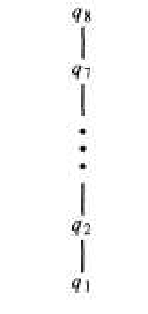
\includegraphics[width=1\linewidth]{images/fig-sol-6-3-11.png}
\end{figure}
%
\end{enumerate}
%
\end{exercisegroup}
\par\smallskip\noindent
\hypertarget{exercisegroup-7}{}\typeout{************************************************}
\typeout{Introduction  }
\typeout{************************************************}
C Exercises%
\begin{exercisegroup}
\item[12.]\hypertarget{exercise-6-3-12}{}Let \(S = \{1,2,3,4,5,6,7\}\) be a poset \((S, \leq )\) with the Hasse diagram shown below. Another relation \(r \subseteq  S\times S\) is defined as follows: \((x, y) \in  r\) if and only if there exists \(z \in S\) such that \(z < x\) and \(z < y\) in the poset \((S, \leq )\).%
\par
\leavevmode%
\begin{enumerate}[label=\alph*]
\item\hypertarget{li-85}{} Prove that \(r\) is reflexive.%
\item\hypertarget{li-86}{} Prove that \(r\) is symmetric.%
\item\hypertarget{li-87}{} A compatible with respect to relation \(r\) is any subset \(Q\) of set \(S\) such that \(x \in  Q \textrm{ and } y \in Q \Rightarrow  (x, y) \in r\). A compatible \(g\) is a maximal compatible if \(Q\) is not a proper subset of another compatible. Give all maximal compatibles with respect to relation \(r\) defined above.%
\item\hypertarget{li-88}{} Discuss a characterization of the set of maximal compatibles for relation \(r\) when \((S, \leq )\) is a general finite poset. What conditions, if any, on a general finite poset \((S, \leq )\) will make r an equivalence relation?%
\end{enumerate}
%
\leavevmode%
\begin{figure}
\centering
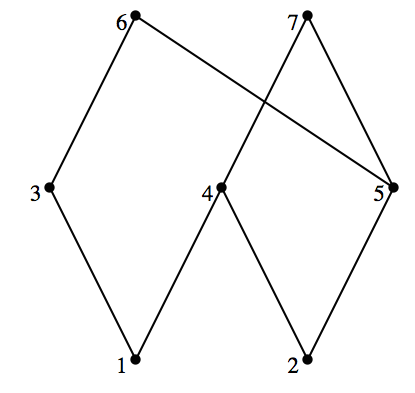
\includegraphics[width=1\linewidth]{images/exercise-6-12.png}
\caption{Hasse diagram for \(r\) in \hyperlink{exercise-6-3-12}{Exercise~1.3.4.12}
                \label{fig-exercise-6-12}}
\end{figure}
\par\smallskip
\end{exercisegroup}
\par\smallskip\noindent
\typeout{************************************************}
\typeout{Section 1.4 Matrices of Relations}
\typeout{************************************************}
\section[Matrices of Relations]{Matrices of Relations}\label{s-matrices-of-relations}
We have discussed two of the many possible ways of representing a relation, namely as a digraph or as a set of ordered pairs. In this section we will discuss the representation of relations by matrices.%
\begin{definition}[Adjacency Matrix]\label{def-adjacency-matrix}
\index{Adjacency Matrix}Let \(A = \{a_1,a_2,\ldots , a_m\}\) and \(B= \{b_1,b_2,\ldots , b_n\}\) be finite sets of cardinality \(m\) and \(n\), respectively. Let \(r\) be a relation from \(A\) into \(B\). Then \(r\) can be represented by the \(m\times n\) matrix \(R\) defined by

\begin{equation*}R_{ij}= \left\{
		\begin{array}{cc}
		 1 & \textrm{   if } a_i r b_j \\
		 0 & \textrm{   otherwise}     \\
		\end{array}\right.
\end{equation*}
 \(R\) is called the \terminology{adjacency matrix} (or the relation matrix) of \(r\).%
\end{definition}
\par
For example, let \(A = \{2, 5, 6\}\) and let \(r\) be the relation \(\{(2, 2), (2, 5), (5, 6), (6, 6)\}\) on \(A\). Since \(r\) is a relation from \(A\) into the same set \(A\) (the \(B\) of the definition), we have \(a_1= 2\), \(a_2=5\), and \(a_3=6\), while \(b_1= 2\), \(b_2=5\), and \(b_3=6\). Next, since%
\par
\leavevmode%
\begin{itemize}[label=\textbullet]
\item{}\(2 r 2\), we have \(R_{11}= 1\)%
\item{}\(2 r 5\), we have \(R_{12}= 1\)%
\item{}\(5 r 6\), we have \(R_{23}= 1\) %
\item{}\(6 r 6\), we have \(R_{33}= 1\)%
\end{itemize}
%
\par
All other entries of \(R\) are zero, so

\(R =\left(
\begin{array}{ccc}
 1 & 1 & 0 \\
 0 & 0 & 1 \\
 0 & 0 & 1 \\
\end{array}
\right)\)
%
\par
From the definition of \(r\) and of composition, we note that

\begin{equation*}r^2 = \{(2, 2), (2, 5), (2, 6), (5, 6), (6, 6)\}\end{equation*}

The adjacency matrix of \(r^2\) is

\begin{equation*}R^2 =\left(
\begin{array}{ccc}
 1 & 1 & 1 \\
 0 & 0 & 1 \\
 0 & 0 & 1 \\
\end{array}
\right)\end{equation*}%
\par
We do not write \(R^2\) only for notational purposes. In fact, \(R^2\) can be obtained from the matrix product \(R R\); however, we must use a slightly different form of arithmetic.%
\begin{definition}[Boolean Arithmetic]\label{def-boolean-arithmetic}
\index{Boolean Arithmetic}Boolean arithmetic is the arithmetic defined on \(\{0,1\}\) using Boolean addition and Boolean multiplication, defined by%
\leavevmode%
\begin{table}
\centering
\begin{tabular}{lll}
\(0 + 0 = 0\)&\(0+1 = 1 + 0=1\)     &\(1 + 1 = 1\)\tabularnewline[0pt]
\(0\cdot 0=0\) & \(0 \cdot  1 = 1 \cdot  0 = 0\)&\(1 \cdot  1 = 1\)
\end{tabular}
\end{table}
\end{definition}
\par
Notice that from Chapter 3, this is the ``arithmetic of logic,'' where \(+\) replaces ``or'' and \(\cdot\) replaces ``and.''%
\begin{example}[Composition by Multiplication]\label{ex-composition-matrices}
If  \(R=\left(
\begin{array}{cccc}
 0 & 1 & 0 & 0 \\
 1 & 0 & 1 & 0 \\
 0 & 1 & 0 & 1 \\
 0 & 0 & 1 & 0 \\
\end{array}
\right)\)  and  \(S=\left(
\begin{array}{cccc}
 0 & 1 & 1 & 1 \\
 0 & 0 & 1 & 1 \\
 0 & 0 & 0 & 1 \\
 0 & 0 & 0 & 0 \\
\end{array}
\right)\).

Then using Boolean arithmetic, \(R S =\left(
\begin{array}{cccc}
 0 & 0 & 1 & 1 \\
 0 & 1 & 1 & 1 \\
 0 & 0 & 1 & 1 \\
 0 & 0 & 0 & 1 \\
\end{array}
\right)\)  and \(S R=\left(
\begin{array}{cccc}
 1 & 1 & 1 & 1 \\
 0 & 1 & 1 & 1 \\
 0 & 0 & 1 & 0 \\
 0 & 0 & 0 & 0 \\
\end{array}
\right)\).
%
\end{example}
\begin{theorem}[Composition is Matrix Multiplication]\label{theorem-composition-is-multiplication}
Let \(A_1\), 
\(A_2\), and \(A_3\) be finite sets where \(r_1\) is a relation from \(A_1\) into \(A_2\) and \(r_2\)
is a relation from \(A_2\) into \(A_3\). If \(R_1\) and \(R_2\) are the adjacency matrices of \(r_1\) and \(r_2\) , respectively, then the product
\(R_1R_2\) using Boolean arithmetic is the adjacency matrix of the composition \(r_1r_2\).%
\end{theorem}
\par
Remark: A convenient help in constructing the adjacency matrix of a relation from a set \(A\) into a set \(B\) is to write the elements from \(A\) in a column preceding the first column of the adjacency matrix, and the elements of \(B\) in a row above the first row. Initially, \(R\) in Example 6.4.1 would be

\begin{equation*}
\begin{array}{cc}
   & 
\begin{array}{ccc}
 2 & 5 & 6 \\
\end{array}
 \\
 
\begin{array}{c}
 2 \\
 5 \\
 6 \\
\end{array}
 & \left(
\begin{array}{ccc}
   &   &   \\
   &   &   \\
   &   &   \\
\end{array}
\right) \\
\end{array}\end{equation*} 

To fill in the matrix, \(R_{ij}\) is 1 if and only if\(\left(a_i,b_j\right) \in r\). So that, since the pair \((2, 5) \in r\), the entry of \(R\) corresponding to the row labeled 2 and the column labeled 5 in the matrix is a 1.%
\begin{example}[Relations and Information]\label{ex-relations-information}
This final example gives an insight into how relational data base programs can systematically answer questions pertaining to large masses of information. Matrices \(R\) (on the left) and \(S\) (on the right) define the relations \(r\) and \(s\) where
\(a r b\) if software \(a\) can be run with operating system \(b\), and \(b s c\) if operating system \(b\) can run on computer \(c\).

\begin{equation*}\begin{array}{cc}
   & 
\begin{array}{cccc}
 \text{OS1} & \text{OS2} & \text{OS3} & \text{OS4} \\
\end{array}
 \\ 
\begin{array}{c}
 \text{P1} \\
 \text{P2} \\
 \text{P3} \\
 \text{P4} \\
\end{array}
 & \left(
\begin{array}{cccc}
  1  &  0  &  1  &  0  \\
  1  &  1  & 0 & 0 \\
 0 & 0 & 0 &  1  \\
 0 & 0 &  1  &  1  \\
\end{array}
\right) \\
\end{array}\)       \(\begin{array}{cc}
   & 
\begin{array}{ccc}
 \text{C1} & \text{C2} & \text{C3} \\
\end{array}
 \\
 
\begin{array}{c}
 \text{OS1} \\
 \text{OS2} \\
 \text{OS3} \\
 \text{OS4} \\
\end{array}
 & \left(
\begin{array}{ccc}
  1  &  1  & 0 \\
 0 &  1  & 0 \\
 0 & 0 &  1  \\
 0 &  1  &  1  \\
\end{array}
\right) \\
\end{array}\end{equation*}

Although the relation between the software and computers is not implicit from the data given, we can easily compute this information. The matrix of \(rs\) is \(RS\), which is

 \begin{equation*}\begin{array}{cc}
   & 
\begin{array}{ccc}
 \text{C1} & \text{C2} & \text{C3} \\
\end{array}
 \\
 
\begin{array}{c}
 \text{P1} \\
 \text{P2} \\
 \text{P3} \\
 \text{P4} \\
\end{array}
 & \left(
\begin{array}{ccc}
  1  &  1  & 1 \\
 1 &  1  & 0 \\
 1 & 1 &  1  \\
 0 &  1  &  1  \\
\end{array}
\right) \\
\end{array}\end{equation*}
This matrix tells us at a glance which software will run on the computers listed. In this case, all software will run on all computers with the exception of program P2, which will not run on the computer C3, and program P4, which will not run on the computer C1.%
\end{example}
\typeout{************************************************}
\typeout{Exercises 1.4.1 Exercises}
\typeout{************************************************}
\subsection[Exercises]{Exercises}\label{exercises-6-4}
\hypertarget{exercisegroup-8}{}\typeout{************************************************}
\typeout{Introduction  }
\typeout{************************************************}
A Exercises%
\begin{exercisegroup}
\item[1.]\hypertarget{exercise-25}{}Let \(A_1 = \{1,2, 3, 4\}\), \(A_2 = \{4, 5, 6\}\), and \(A_3 = \{6, 7, 8\}\). Let \(r_1\) be the relation from \(A_1\) into \(A_2\) defined by
\(r_1 = \{(x, y)  \mid  y - x = 2\}\), and let \(r_2\) be the relation from \(A_2\) into \(A_3\) defined by \(r_2 = \{(x, y) \mid  y - x = 1\}\).%
\par
\leavevmode%
\begin{enumerate}[label=\alph*]
\item\hypertarget{li-93}{} Determine the adjacency matrices of \(r_1\) and \(r_2\).%
\item\hypertarget{li-94}{} Use the definition of composition to find \(r_1r_2\).%
\item\hypertarget{li-95}{} Verify the result in part by finding the product of the adjacency matrices of \(r_1\) and \(r_2\).%
\end{enumerate}
%
\par\smallskip
\par\smallskip
\noindent\textbf{Answer.}\hypertarget{answer-13}{}\quad
\leavevmode%
\begin{enumerate}[label=\alph*]
\item\hypertarget{li-96}{} \(\begin{array}{cc}
   & 
\begin{array}{ccc}
 4 & 5 & 6 \\
\end{array}
 \\
 
\begin{array}{c}
 1 \\
 2 \\
 3 \\
 4 \\
\end{array}
 & \left(
\begin{array}{ccc}
 0 & 0 & 0 \\
 1 & 0 & 0 \\
 0 & 1 & 0 \\
 0 & 0 & 1 \\
\end{array}
\right) \\
\end{array}\)  and \(\begin{array}{cc}
   & 
\begin{array}{ccc}
 6 & 7 & 8 \\
\end{array}
 \\
 
\begin{array}{c}
 4 \\
 5 \\
 6 \\
\end{array}
 & \left(
\begin{array}{ccc}
 0 & 0 & 0 \\
 1 & 0 & 0 \\
 0 & 1 & 0 \\
\end{array}
\right) \\
\end{array}\)%
\item\hypertarget{li-97}{}\( r_1r_2 =\{(3,6),(4,7)\}\)%
\item\hypertarget{li-98}{} \(\begin{array}{cc}
   & 
\begin{array}{ccc}
 6 & 7 & 8 \\
\end{array}
 \\
 
\begin{array}{c}
 1 \\
 2 \\
 3 \\
 4 \\
\end{array}
 & \left(
\begin{array}{ccc}
 0 & 0 & 0 \\
 0 & 0 & 0 \\
 1 & 0 & 0 \\
 0 & 1 & 0 \\
\end{array}
\right) \\
\end{array}\)
%
\end{enumerate}
%
\item[2.]\hypertarget{exercise-26}{}\leavevmode%
\begin{enumerate}[label=\alph*]
\item\hypertarget{li-99}{} Determine the adjacency matrix of each relation given via the digraphs in Exercise 3 of Section 6.3.%
\item\hypertarget{li-100}{} Using the matrices found in part (a) above, find \(r^2\) of each relation in Exercise 3 of Section 6.3.%
\item\hypertarget{li-101}{} Find the digraph of \(r^2\) directly from the given digraph and compare your results with those of part (b).%
\end{enumerate}
%
\par\smallskip
\item[3.]\hypertarget{exercise-27}{}Suppose that the matrices in \hyperref[ex-composition-matrices]{Example~\ref{ex-composition-matrices}} are relations on \(\{1, 2, 3, 4\}\). What relations do \(R\) and \(S\) describe?%
\par\smallskip
\par\smallskip
\noindent\textbf{Answer.}\hypertarget{answer-14}{}\quad
\leavevmode%
\begin{table}
\centering
\begin{tabular}{l}
R : \(x r y\) if and only if \( \lvert x -y \rvert = 1\)\tabularnewline[0pt]
S : \(x s y\) if and only if \(x\) is less than \(y\). 
\end{tabular}
\end{table}
\item[4.]\hypertarget{exercise-28}{}Let \(D\) be the set of weekdays, Monday through Friday, let \(W\) be a set of employees \(\{1, 2, 3\}\) of a tutoring center, and let \(V\) be a set
of computer languages for which tutoring is offered,  \(\{A(PL), B(asic), C(++), J(ava), L(isp), P(ython)\}\). We define \(s\) (schedule)
from \(D\) into \(W\) by \(d s w\) if \(w\) is scheduled to work on day \(d\). We also define \(r\) from \(W\)
into \(V\) by \(w r l\) if \(w\) can tutor students in language \(l\). If \(s\) and \(r\) are defined by matrices%
\par

\begin{equation*} 
S = 
\begin{array}{cc}
   & 
		\begin{array}{ccc}
		1 & 2 & 3 \\
		\end{array}
		 \\
 
	\begin{array}{c}
			 M \\
			 T \\
			 W \\
			 R \\
			 F \\
	\end{array}
     & 
     \left(
			\begin{array}{ccc}
				 1 & 0 & 1 \\
				 0 & 1 & 1 \\
				 1 & 0 & 1 \\
				 0 & 1 & 0 \\
				 1 & 1 & 0 \\
			\end{array}
		\right) \\
		\end{array}
\textrm{ and }R=
	\begin{array}{cc}
   & 
	\begin{array}{cccccc}
		 A & B & C & J & L & P \\
	\end{array}
 \\
 
\begin{array}{c}
 1 \\
 2 \\
 3 \\
\end{array}
 & \left(
\begin{array}{cccccc}
 0 & 1 & 1 & 0 & 0 & 1 \\
 1 & 1 & 0 & 1 & 0 & 1 \\
 0 & 1 & 0 & 0 & 1 & 1 \\
\end{array}
\right) \\
\end{array}\end{equation*}
%
\par
\leavevmode%
\begin{enumerate}[label=\alph*]
\item\hypertarget{li-102}{} compute \(S R\) using Boolean arithmetic and give an interpretation of the relation it defines, and%
\item\hypertarget{li-103}{} compute \(S R\) using regular arithmetic and give an interpretation of what the result describes.%
\end{enumerate}
%
\par\smallskip
\item[5.]\hypertarget{exercise-29}{} How many different reflexive, symmetric relations are there on a set with three elements?%
\par\smallskip
\par\smallskip
\noindent\textbf{Hint.}\hypertarget{hint-1}{}\quad
Consider the possible matrices.%
\par\smallskip
\noindent\textbf{Answer.}\hypertarget{answer-15}{}\quad
 The diagonal entries of the matrix for such a relation must be 1. When the three entries above the diagonal are determined, the entries below are also determined. Therefore, there are \(2^3\) fitting the description.%
\item[6.]\hypertarget{exercise-30}{}Let \(A = \{a, b, c, d\}\).  Let \(r\) be the relation on \(A\) with adjacency matrix

\(\begin{array}{cc}
   & 
\begin{array}{cccc}
 a & b & c & d \\
\end{array}
 \\
 
\begin{array}{c}
 a \\
 b \\
 c \\
 c \\
\end{array}
 & \left(
\begin{array}{cccc}
 1 & 0 & 0 & 0 \\
 0 & 1 & 0 & 0 \\
 1 & 1 & 1 & 0 \\
 0 & 1 & 0 & 1 \\
\end{array}
\right) \\
\end{array}\)%
\par
\leavevmode%
\begin{enumerate}[label=\alph*]
\item\hypertarget{li-104}{} Explain why \(r\) is a partial ordering on \(A\).%
\item\hypertarget{li-105}{} Draw its Hasse diagram.%
\end{enumerate}
%
\par\smallskip
\item[7.]\hypertarget{exercise-31}{}Define relations \(p\) and \(q\) on \(\{1, 2, 3, 4\}\) by \(p = \{(a, b) \mid \lvert a-b\rvert=1\}\) and \(q=\{(a,b) \mid a-b \textrm{ is even}\}\).%
\par
\leavevmode%
\begin{enumerate}[label=\alph*]
\item\hypertarget{li-106}{} Represent \(p\) and \(q\) as both graphs and matrices.%
\item\hypertarget{li-107}{} Determine \(p q\), \(p^2\), and \(q^2\); and represent them clearly in any way.%
\end{enumerate}
%
\par\smallskip
\par\smallskip
\noindent\textbf{Answer.}\hypertarget{answer-16}{}\quad
\leavevmode%
\begin{enumerate}[label=\alph*]
\item\hypertarget{li-108}{} \(\begin{array}{cc}
  & 
\begin{array}{cccc}
 1 & 2 & 3 & 4 \\
\end{array}
 \\
 
\begin{array}{c}
 1 \\
 2 \\
 3 \\
 4 \\
\end{array}
 & \left(
\begin{array}{cccc}
 0 & 1 & 0 & 0 \\
 1 & 0 & 1 & 0 \\
 0 & 1 & 0 & 1 \\
 0 & 0 & 1 & 0 \\
\end{array}
\right) \\
\end{array}\) and \(\begin{array}{cc}
   & 
\begin{array}{cccc}
 1 & 2 & 3 & 4 \\
\end{array}
 \\
 
\begin{array}{c}
 1 \\
 2 \\
 3 \\
 4 \\
\end{array}
 & \left(
\begin{array}{cccc}
 1 & 0 & 1 & 0 \\
 0 & 1 & 0 & 1 \\
 1 & 0 & 1 & 0 \\
 0 & 1 & 0 & 1 \\
\end{array}
\right) \\
\end{array}\)%
\item\hypertarget{li-109}{}  \(P Q=
\begin{array}{cc}
   & 
\begin{array}{cccc}
 1 & 2 & 3 & 4 \\
\end{array}
 \\
 
\begin{array}{c}
 1 \\
 2 \\
 3 \\
 4 \\
\end{array}
 & \left(
\begin{array}{cccc}
 0 & 1 & 0 & 0 \\
 1 & 0 & 1 & 0 \\
 0 & 1 & 0 & 1 \\
 0 & 0 & 1 & 0 \\
\end{array}
\right) \\
\end{array}\)

 \(P^2 =\text{  }
\begin{array}{cc}
   & 
\begin{array}{cccc}
 1 & 2 & 3 & 4 \\
\end{array}
 \\
 
\begin{array}{c}
 1 \\
 2 \\
 3 \\
 4 \\
\end{array}
 & \left(
\begin{array}{cccc}
 0 & 1 & 0 & 0 \\
 1 & 0 & 1 & 0 \\
 0 & 1 & 0 & 1 \\
 0 & 0 & 1 & 0 \\
\end{array}
\right) \\
\end{array}\)\(=Q^2\)
%
\end{enumerate}
%
\end{exercisegroup}
\par\smallskip\noindent
\hypertarget{exercisegroup-9}{}\typeout{************************************************}
\typeout{Introduction  }
\typeout{************************************************}
B Exercises%
\begin{exercisegroup}
\item[8.]\hypertarget{exercise-32}{}\leavevmode%
\begin{enumerate}[label=\alph*]
\item\hypertarget{li-110}{}Prove that if \(r\) is a transitive relation on a set \(A\), then \(r^2 \subseteq  r\). %
\item\hypertarget{li-111}{} Find an example of a transitive relation for which \(r^2\neq r\).%
\end{enumerate}
%
\par\smallskip
\item[9.]\hypertarget{exercise-33}{} We define \(\leq\) on the set of all \(n\times n\) relation matrices by the rule that if \(R\) and \(S\) are any two \(n\times n\)
relation matrices, \(R \leq  S\) if and only if \(R_{ij} \leq S_{ij}\) for all \(1 \leq  i, j \leq  n\).%
\par
\leavevmode%
\begin{enumerate}[label=\alph*]
\item\hypertarget{li-112}{} Prove that \(\leq\) is a partial ordering on all \(n\times n\) relation matrices.%
\item\hypertarget{li-113}{} Prove that \(R \leq  S  \Rightarrow   R^2\leq S^2\) , but the converse is not true.%
\item\hypertarget{li-114}{} If \(R\) and \(S\) are matrices of equivalence relations and \(R \leq  S\), how are the equivalence classes defined by \(R\) related to the equivalence classes defined by \(S\)?%
\end{enumerate}
%
\par\smallskip
\par\smallskip
\noindent\textbf{Answer.}\hypertarget{answer-17}{}\quad
\leavevmode%
\begin{enumerate}[label=\alph*]
\item\hypertarget{li-115}{}Reflexive: \(R_{ij}=R_{ij}\) for all \(i,j\), therefore \(R_{ij}\leq R_{ij}\)%
\par
 Antisymmetric: Assume \(R_{ij}\leq S_{ij}\) and \(S_{ij}\leq R_{ij}\) for all \(1\leq i,j\leq n\). Therefore, \(R_{ij} = S_{ij}\) for all \(1\leq i,j\leq n\)  and so \(R=S\)%
\par
Transitive: Assume \(R, S,\) and \(T\) are matrices where \(R_{ij}\leq S_{ij}\) and \(S_{ij}\leq T_{ij}\), for all \(1\leq i,j\leq n\). Then \(R_{ij}\leq T_{ij}\) for all \(1\leq i,j\leq n\), and so \(R\leq T\).%
\item\hypertarget{li-116}{}\begin{equation*}
\begin{split}
 \left(R^2\right)_{ij}&=R_{i1}R_{1j}+R_{i2}R_{2j}+\cdots +R_{in}R_{nj}\\
       &\leq S_{i1}S_{1j}+S_{i2}S_{2j}+\cdots +S_{in}S_{nj}\\
       &=\left(S^2\right)_{ij} \Rightarrow R^2\leq S^2
\end{split}
\end{equation*}%
\par
To verify that the converse is not true we need only one example. For \(n=2\), let \(R_{12}=1\) and all other entries equal \(0\), and let \(S\) be the zero matrix. Since \(R^2\) and \(S^2\) are both the zero matrix, \(R^2\leq S^2\), but since \(R_{12}>S_{12}, R\leq S\) is false.%
\item\hypertarget{li-117}{} The matrices are defined on the same set \(A=\left\{a_1,a_2,\ldots  ,a_n\right\}\). Let \(c\left(a_i\right), i=1,2,\ldots  ,n\) be the equivalence classes defined by \(R\) and let \(d\left(a_i\right)\) be those defined by \(S\). Claim: \(c\left(a_i\right)\subseteq d\left(a_i\right)\). 
	\begin{equation*}\begin{split}
	 a_j\in c\left(a_i\right)&\Rightarrow a_i r a_j\\
	 		&\Rightarrow R_{ij}=1 \Rightarrow S_{ij}=1\\
	 		&\Rightarrow a_i s a_j\\ 
	 		& \Rightarrow a_j \in d\left(a_i\right)\\
	 		\end{split}
	 \end{equation*}%
\end{enumerate}
%
\end{exercisegroup}
\par\smallskip\noindent
\typeout{************************************************}
\typeout{Section 1.5 Closure Operations on Relations}
\typeout{************************************************}
\section[Closure Operations on Relations]{Closure Operations on Relations}\label{s-closure-operations-on-relations}
In Section 6.1, we studied relations and one important operation on relations, namely composition. This operation enables us to generate new relations from previously known relations. In Section 6.3, we discussed some key properties of relations. We now wish to consider the situation of constructing a new relation \(r^+\) from an existing relation \(r\) where, first, \(r^+\) contains \(r\) and, second, \(r^{+ }\) satisfies the transitive property.%
\par
Consider a telephone network in which the main office \(a\) is connected to, and can communicate to, individuals \(b\) and \(c\).  Both \(b\) and \(c\) can communicate to another person, \(d\); however, the main office cannot communicate with \(d\). Assume communication is only one way, as indicated. This situation can be described by the relation \(r = \{(a, b), (a, c), (b, d), (c, d)\}\). We would like to change the system so that the main office \(a\) can communicate with person \(d\) and still maintain the previous system. We, of course, want the most economical system.%
\par
This can be rephrased as follows; Find the smallest relation \(r^{+ }\)which contains \(r\) as a subset and which is transitive; \(r^+ =\{(a, b), (a, c), (b, d), (c, d), (a, d)\}\).%
\begin{definition}[Transitive Closure]\label{def-transitive-closure}
\index{Transitive Closure}\label{notation-6}
Let \(A\) be a set and \(r\) be a relation on \(A\). The transitive closure of \(r\), denoted by \(r^+\) , is the smallest transitive relation that contains \(r\) as a subset.%
\end{definition}
\par
Let \(A = \{1, 2, 3, 4\}\), and let \(\mathcal{S} = \{(1, 2), (2, 3), (3, 4)\}\) be a relation on \(A\). This relation is called the successor relation on \(A\) since each element is related to its successor. How do we compute \(\mathcal{S}^+\)?  By inspection we note that \((1, 3)\) must be in \(\mathcal{S}^+\) . Let's analyze why. This is so because \((1,2) \in \mathcal{S}\) and \((2, 3) \in \mathcal{S}\), and the transitive property forces \((1,3)\) to be in \(\mathcal{S}^+\). %
\par
In general, it follows that if \((a, b) \in \mathcal{S}\) and \((b, c) \in S,\) then \((a, c) \in \mathcal{S}^+ \). This condition is exactly the membership requirement for the pair \((a, c)\) to be in the composition \(\mathcal{S}\mathcal{S} = \mathcal{S}^2\). So every element in \(\mathcal{S}^2\) must be an element in \(\mathcal{S}^+\) . So we now know that, \(\mathcal{S}^+\) contains at least \(\mathcal{S} \cup  \mathcal{S}^2\) . In particular, for this example, since \(\mathcal{S} = \{(1, 2), (2, 3), (3, 4)\}\) and \(\mathcal{S}^2 = \{(1, 3), (2, 4)\}\), we have 

\[\mathcal{S} \cup  \mathcal{S}^2 =\{(1, 2), (2, 3), (3, 4), (1, 3), (2, 4)\}\]
%
\par
Is the relation \(\mathcal{S} \cup  \mathcal{S}^2\) transitive? Again, by inspection, \((1, 4)\) is not an element of \(\mathcal{S} \cup  \mathcal{S}^2\), but  \((1,3) \in \mathcal{S}^2\) and \((3, 4) \in \mathcal{S}\). Therefore, the composition \(\mathcal{S}^2 \mathcal{S} = \mathcal{S}^3\) produces \((1, 4)\), and it must be an element of \(\mathcal{S}^+\) since \((1,3)\) and \((3, 4)\) are required to be in \(\mathcal{S}^+\).  This shows that \(\mathcal{S}^3 \subseteq  \mathcal{S} ^+\) . This process must be continued until the resulting relation is transitive. If A is finite, as is true in this example, the transitive closure will be obtained in a finite number of steps. For this example, 

 \[\mathcal{S}^+ =\mathcal{S}\cup \mathcal{S} ^2\cup  \mathcal{S} ^3=\{(1, 2), (2, 3), (3, 4),(1, 3),(2, 4),(1,4)\}\]
 %
\begin{theorem}[Transitive Closure on a Finite Set]\label{theorem-transitive-closure-formula}
If \(r\) is a relation on a set \(A\) and \(\lvert A \rvert = n\), then the transitive closure of \(r\) is the union of the first \(n\) powers of
r.  That is, 
\[r^+ = r \cup  r^2 \cup  r ^3 \cup \cdots  \cup  r^n\].%
\end{theorem}
\par
Let's now consider the matrix analogue of the transitive closure.%
\par
Consider the relation 

\(r = \{(1, 4), (2, 1), (2, 2), (2, 3),(3, 2), (4, 3), (4, 5), (5, 1)\}\) 

on the set \(A = \{1,2, 3, 4, 5\}\). The matrix of \(r\) is



 \(R=\left(
\begin{array}{ccccc}
 0 & 0 & 0 & 1 & 0 \\
 1 & 1 & 1 & 0 & 0 \\
 0 & 1 & 0 & 0 & 0 \\
 0 & 0 & 1 & 0 & 1 \\
 1 & 0 & 0 & 0 & 0 \\
\end{array}
\right)\)%
\par
Recall that \(r^2, r^3, \ldots\)  can be determined through computing the matrix powers \(R^2, R^3, \ldots\).  For our example,%
\leavevmode%
\begin{table}
\centering
\begin{tabular}{ll}

 \(R^2=\left(
\begin{array}{ccccc}
 0 & 0 & 1 & 0 & 1 \\
 1 & 1 & 1 & 1 & 0 \\
 1 & 1 & 1 & 0 & 0 \\
 1 & 1 & 0 & 0 & 0 \\
 0 & 0 & 0 & 1 & 0 \\
\end{array}
\right)\) & \(R^3=\left(
\begin{array}{ccccc}
 1 & 1 & 0 & 0 & 0 \\
 1 & 1 & 1 & 1 & 1 \\
 1 & 1 & 1 & 1 & 0 \\
 1 & 1 & 1 & 1 & 0 \\
 0 & 0 & 1 & 0 & 1 \\
\end{array}
\right)\)\tabularnewline[0pt]

 \(R^4=\left(
\begin{array}{ccccc}
 1 & 1 & 1 & 1 & 0 \\
 1 & 1 & 1 & 1 & 1 \\
 1 & 1 & 1 & 1 & 1 \\
 1 & 1 & 1 & 1 & 1 \\
 1 & 1 & 0 & 0 & 0 \\
\end{array}
\right)\)&\(R^5=\left(
\begin{array}{ccccc}
 1 & 1 & 1 & 1 & 1 \\
 1 & 1 & 1 & 1 & 1 \\
 1 & 1 & 1 & 1 & 1 \\
 1 & 1 & 1 & 1 & 1 \\
 1 & 1 & 1 & 1 & 0 \\
\end{array}
\right)\)
\end{tabular}
\end{table}
\par
How do we relate \(\underset{i=1}{\overset{5}{\cup }}r^i\) to the powers of \(R\)?%
\begin{theorem}[Matrix of a Transitive Closure]\label{theorem-matrix-transitive-closure}
Let \(r\) be a relation on a finite set and let \(R^+\) be the matrix of \(r^+\) , the transitive closure of \(r\).  Then \(R^+
= R + R^2 + \cdots + R^n\), using Boolean arithmetic.%
\end{theorem}
\par
Using this theorem, we find \(R^+\) is the \(5\times 5\) matrix consisting of all \(1's\), thus, \(r^+\) is all of \(A \times A\).%
\par
Let \(r\) be a relation on the set \(\{1, 2, \dots , n\}\) with relation matrix \(R\). The matrix of the transitive closure \(R^+\), can be computed by the equation \(R^+ = R + R ^2 + \cdots  + R^n\). By using ordinary polynomial evaluation methods, you can compute \(R^+\) with \(n -1\) matrix multiplications: 
\[R^+ = R(I + R(I +( \cdots  R(I+ R) \cdots )))\]%
\par
For example, if \(n = 3\), \(R = R(I + R(I + R))\).%
\par
We can make use of the fact that if \(T\) is a relation matrix, \(T + T = T\) due to the fact that \(1 + 1 = 1\) in Boolean arithmetic. Let \(S_k = R + R^2 + \cdots  + R^k\) . Then %
\par
\begin{equation*}
\begin{split}
R &= S_1\\
S_1(I+S_1)&=R(I+R)=R+R^2 = S_2 \\
S_2(I+S_2)&=(R+R^2)(I+R+R^2) \\
			&=(R+R^2)+(R^2+R^3)+(R^3+R^4) \\
			&=R+R^2+R^3+R^4 = S_4 
\end{split}
\end{equation*}%
\par
Similarly,
\[S_4(I+S_4)=S_8\]
and by induction we can prove
\[S_{2^k}(I+S_{2^k})=S_{2^{k+1}}\]
%
\par
Notice how each matrix multiplication doubles the number of terms that have been added to the sum that you currently have computed. In algorithmic form, we can compute \(R^+\) as follows.%
\begin{algorithm}[Transitive Closure Algorithm]\label{alg-trans-closure}
 Let \(R\) be a relation matrix and let \(R^+\) be its transitive closure matrix, which is to be computed as matrix \(T\)%
\begin{lstlisting}[style=genericinput]
1.0. S = R
2.0  T= S*(I+S)
3.0 While T != S
		3.1 S = T
		3.2 T= S*(I+S) // using Boolean arithmetic
4.0 Return T
\end{lstlisting}
\end{algorithm}
\begin{note}[]\label{note-1}
\leavevmode%
\begin{itemize}[label=\textbullet]
\item{} Often the higher-powered terms in \(S_n\) do not contribute anything to \(R^+\). When the condition \(T = S\) becomes true in Step 3, this is an indication that no higher-powered terms are needed.%
\item{} To compute \(R^+\) using this algorithm, you need to perform no more than \(\lceil \log_2 n \rceil\) matrix multiplications, where
\(\lceil x \rceil\) is the least integer that is greater than or equal to \(x\). For example, if \(r\) is a relation on 25 elements,
no more than \(\lceil \log_2 25 \rceil = 5\) matrix multiplications are needed.%
\end{itemize}
%
\end{note}
\par
A second algorithm, Warshall's Algorithm, reduces computation time to the time that it takes to perform one matrix multiplication.%
\begin{algorithm}[Warshall's Algorithm]\label{alg-warshall}
Let \(R\) be an \(n \times n\) relation matrix and let \(R^+\) be its transitive closure matrix, which is to be computed as matrix \(T\) using boolean arithmetic%
\begin{lstlisting}[style=genericinput]
1.0 T = R
2.0 for k = 1 to n:
     for i = 1 to n:
      for j = 1 to n:
        T[i,j]= T[i,j] + T[i,k] * T[k,j]
3.0 Return T
\end{lstlisting}
\end{algorithm}
\typeout{************************************************}
\typeout{Exercises 1.5.1 Exercises}
\typeout{************************************************}
\subsection[Exercises]{Exercises}\label{exercises-6-5}
\hypertarget{exercisegroup-10}{}\typeout{************************************************}
\typeout{Introduction  }
\typeout{************************************************}
A Exercises%
\begin{exercisegroup}
\item[1.]\hypertarget{exercise-34}{} Let \(A\) and \(\mathcal{S}\) be as defined above. Compute \(\mathcal{S}^+\) using the matrix representation of \(\mathcal{S}\). Verify your results by checking against the result obtained directly from the definition of transitive closure.%
\par\smallskip
\item[2.]\hypertarget{exercise-35}{}Let \(A=\{1,2,3,4,6,12\}\) and \(t=\{(a,b)\mid b/a \textrm{ is a prime number}\}\). determine \(t^+\) by any means but represent it as a matrix.%
\par\smallskip
\item[3.]\hypertarget{exercise-36}{}\leavevmode%
\begin{enumerate}[label=\alph*]
\item\hypertarget{li-120}{}Draw digraphs of the relations \(\mathcal{S}\), \(\mathcal{S}^2\), \(\mathcal{S}^3\) , and \(\mathcal{S}^+\)  where \(\mathcal{S}\) is defined above.%
\item\hypertarget{li-121}{} Verify that in terms of the graph of \(\mathcal{S}\), \(a \mathcal{S}^+ b\) if and only if \(b\) is reachable from \(a\) along a
path of any finite nonzero length.%
\end{enumerate}
%
\par\smallskip
\par\smallskip
\noindent\textbf{Answer.}\hypertarget{answer-18}{}\quad
\leavevmode%
\begin{enumerate}[label=\alph*]
\item\hypertarget{li-122}{}\leavevmode%
\begin{figure}
\centering
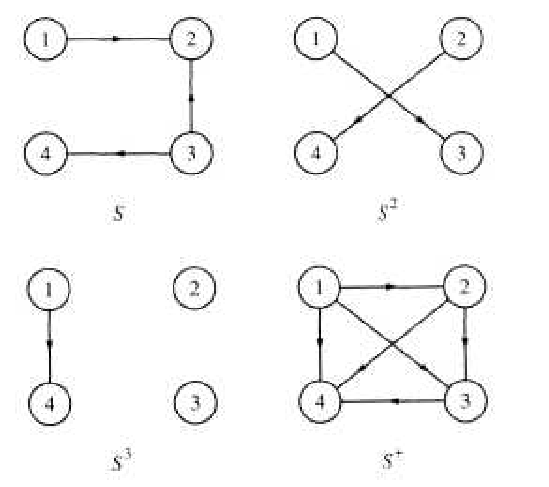
\includegraphics[width=1\linewidth]{images/fig-sol-6-5-3.png}
\end{figure}
%
\item\hypertarget{li-123}{}  Example, \(1s 4\) and using \(S\) one can go from 1 to 4 using a path of length 3.%
\end{enumerate}
%
\item[4.]\hypertarget{exercise-37}{} Let \(r\) be the relation represented by the following digraph.%
\par
\leavevmode%
\begin{enumerate}[label=\alph*]
\item\hypertarget{li-124}{} Find \(r^+\) using the definition based on order pairs.%
\item\hypertarget{li-125}{} Determine the digraph of \(r^+\) directly from the digraph of \(r\).%
\item\hypertarget{li-126}{} Verify your result in part (b) by computing the digraph from your result in part (a).%
\end{enumerate}
%
\leavevmode%
\begin{figure}
\centering
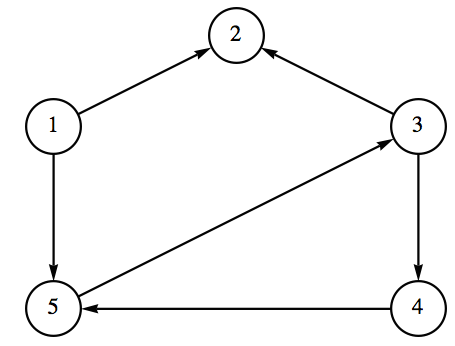
\includegraphics[width=1\linewidth]{images/fig-exercise-6-5-4.png}
\caption{Digraph of \(r\) in exercise 4. 
			 \label{figure-18}}
\end{figure}
\par\smallskip
\item[5.]\hypertarget{exercise-38}{}\leavevmode%
\begin{enumerate}[label=\alph*]
\item\hypertarget{li-127}{}Define reflexive closure and symmetric closure by imitating the definition of transitive closure.%
\item\hypertarget{li-128}{} Use your definitions to compute the reflexive and symmetric closures of examples in the text.%
\item\hypertarget{li-129}{} What are the transitive reflexive closures of these examples?%
\item\hypertarget{li-130}{} Convince yourself that the reflexive closure of the relation \(<\) on the set of positive integers \(\mathbb{P}\) is \(\leq\).%
\end{enumerate}
%
\par\smallskip
\par\smallskip
\noindent\textbf{Answer.}\hypertarget{answer-19}{}\quad
Definition: Reflexive Closure.  Let \(r\) be a relation on \(A\). The reflexive closure of \(r\) is the smallest reflexive relation that contains \(r\).%
\par
Theorem: The reflexive closure of \(r\) is the union of \(r\) with \(\{(x, x) : x\in A\}\) 
%
\item[6.]\hypertarget{exercise-39}{} What common relations on \(\mathbb{Z}\) are the transitive closures of the following relations?%
\par
\leavevmode%
\begin{enumerate}[label=\alph*]
\item\hypertarget{li-131}{} \(a S b\) if and only if \(a + 1 = b\).%
\item\hypertarget{li-132}{} \(a R b\) if and only if \(| a - b | = 2\).%
\end{enumerate}
%
\par\smallskip
\end{exercisegroup}
\par\smallskip\noindent
\hypertarget{exercisegroup-11}{}\typeout{************************************************}
\typeout{Introduction  }
\typeout{************************************************}
B Exercises%
\begin{exercisegroup}
\item[7.]\hypertarget{exercise-40}{}\leavevmode%
\begin{enumerate}[label=\alph*]
\item\hypertarget{li-133}{}Let \(A\) be any set and \(r\) a relation on \(A\), prove that \(\left(r^+\right)^+=r^+\).%
\item\hypertarget{li-134}{}Is the transitive closure of a symmetric relation always both symmetric and reflexive? Explain.%
\end{enumerate}
%
\par\smallskip
\par\smallskip
\noindent\textbf{Answer.}\hypertarget{answer-20}{}\quad
\leavevmode%
\begin{enumerate}[label=\alph*]
\item\hypertarget{li-135}{}  By the definition of transitive closure, \(r^+\) is the smallest relation which contains \(r\); therefore, it is transitive. The transitive closure of \(r^+\), \(\left(r^+\right)^+\) , is the smallest transitive relation that contains \(r^+\). Since \(r^+\) is transitive, \(\left(r^+\right)^+=r^+\). %
\item\hypertarget{li-136}{}  The transitive closure of a symmetric relation is symmetric, but it may not be reflexive. If one element is not related to any elements, then the transitive closure will not relate that element to others.
%
\end{enumerate}
%
\end{exercisegroup}
\par\smallskip\noindent
%
\backmatter
%
%
%% A lineskip in table of contents as transition to appendices, backmatter
\addtocontents{toc}{\vspace{\normalbaselineskip}}
%
\typeout{************************************************}
\typeout{References  References}
\typeout{************************************************}
\chapter[References]{References}\label{references-1}
%% If this is a top-level references
%%   you can replace with "thebibliography" environment
\begin{referencelist}
\bibitem[1]{biblio-sopowit-1983}\hypertarget{biblio-sopowit-1983}{}Sopowit, K. J., E. M. Reingold, and D. A. Plaisted \textit{The Traveling Salesman Problem and Minimum Matching in the Unit Square}.SIAM J. Computing, 1983,\textbf{12}, 144\textendash{}56.
\end{referencelist}
%
%% The index is here, setup is all in preamble
\printindex
%
\end{document}